% !TEX root = ../report.tex

\chapter{State Of The Art}
\minitoc
\label{chap:SotA}

This chapter will present and discuss previous work in the field of recommender
systems. The first section will give the reader an introduction to the field of
recommender systems. The methods described in this section also builds makes up the
fundament which the methods described later in the chapter are built from.
The second section introduces the cold-start problem and presents a handful of existing
solutions to the cold-start problem. The third section explores the fashion domain
and discuss what properties makes it unique in the context of making personalized
recommendations. The section also presents existing fashion recommendation methods. 
Section four explores how user logs can be utilized to provide personalized recommendations.
The last section of the chapter presents different methods and evaluation metrics for measuring
the performance of recommender systems.

\clearpage

% !TEX root = ../../report.tex

\section{Recommender Systems Foundations}
\label{sec:recsys}
Recommender systems have become an important research topic since the
introduction of Tapestry \cite{Goldberg1992}, the first collaborative filtering
system back in 1992. Recommender systems now play an important role in many of
the most popular web-sites such as Amazon, YouTube, Netflix, TripAdvisor,
Last.fm, and IMDb. In its most common formulation the recommendation problem is
reduced to the problem of estimating the preference/rating of items that have
not been seen by a user. Usually, this estimation is based on one or more of
the following assumptions:

\begin{itemize}
\item You are like your friends
\item You are like people who do similar things that you do
\item You like things that are similar to things you already like
\item You are influenced by experts and the opinions of others.
\end{itemize}

Once these ratings have been estimated we can recommend the items with the
highest rating to the user. These recommendations relate to various
decision-making processes, such as what items to buy, what music to listen to,
or what online news to read. Recommender systems are usually classified into
the following categories, based on how the recommendations are made
\cite{Adomavicius2005}.

\begin{itemize}
\item \emph{Content-based recommendations:} The user will be recommended items with similar content to the ones the user preferred in the past;
\item \emph{Collaborative recommendations:} The user will be recommended items that people with similar tastes and preferences have liked in the past;
\item \emph{Hybrid approaches:} These methods combine collaborative and content-based methods.
\end{itemize}

\subsection{Content Based Filtering}

In a content-based system, we must construct a user \emph{profile}
$ContentBasedProfile(c)$ for each user $c$, which is a record or collection of
the attributes which characterizes each item $Content(s)$ of all the items
$s_{i} \epsilon S$ previously rated by user $c$. For example in a fashion
recommender system the content-based recommender system tries to understand the
commonalities among the items user $c$ has rated highly in the past (color,
brand, store, price, etc.). Then recommend items that have a high degree of
similarity to these items. $ContentBasedProfile(c)$ can be designed as a vector
of weights $(w_{c1} ... w_{ck})$, where each weight $w_{ci}$ denotes the
importance of the keyword $k_{i}$ to user $c$.

Figure \ref{figure:contentbaseddb} shows a simple database with rows
describing 5 items that have been rated by 3 users. The column names starting
with $X_{n}$ are the properties of the items, often referred to as
"attributes".

\begin{figure}[H]
    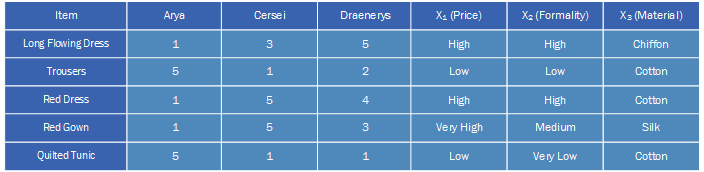
\includegraphics[width=5in]{image/contentbaseddb.png}
    \centering
    \caption[A clothing database]{A clothing database. Rows are items, columns are users and item attributes}
    \label{figure:contentbaseddb}
\end{figure}

From the rating matrix and content properties one can then construct a
$ContentBasedProfile(c)$ for each user $c$, for the user Arya one could imagine
it would look something like this.

\begin{figure}[H]
    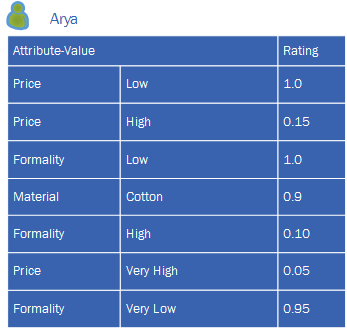
\includegraphics[width=2in]{image/contentprofile.png}
    \centering
    \caption[Content Profile Example]{Content Profile Example}
    \label{figure:contentprofile}
\end{figure}

The recommendation process consists of matching up the attributes of the user
profile against the attributes of an item. The utility function $r(u, i)$ is usually defined as:

\begin{equation}
r(u,i) = score(ContentBasedProfile(u), Content(i)).
\end{equation}

The result is a relevance judgment that represents the user's level of interest
in that object. The utility $u(c,s)$ of item $s$ for user $c$ is estimated based on the utilities $u(c, s_{i})$
assigned by user c to items $s_{i} \epsilon S$ that exhibit a similarity to
item $s$. E.g. for the user Arya items with the attributes low price and low
formality could safely be recommended as they fit her user profile, and have
similar characteristics to the items which she previously have rated highly.

\subsection{Collaborative Filtering}
\label{subsec:cf}

The goal of collaborative filtering methods is to suggest new items or to
predict the utility $u(c, s)$ of a certain item $s$ for a particular user $c$ based
on the user's previous activities and/or likings and similarity to other users~\cite{Sammut:2011:EML:2011878}.
In a typical CF scenario, there is a list of $n$ users $C = {c_{1}, ... c_{n}}$
and a list of $m$ items $S = {s_{1},...s_{m}}$. Each user $c_{i}$ has a list of
items $S_{si}$, which the user have expressed her opinion about, which makes up
our rating matrix of size $S \times C$. More formally, the utility $u(c, s)$ of
item $s$ for user $c$ is estimated based on the utilities $u(c_{j}, s)$
assigned to item $s$ by the users $c_{j} \epsilon C$, which can be considered
"similar" to the active user $c$. This is exemplified in Figure
\ref{figure:ratingmatrix}. For example, in our fashion recommender system, in
order to recommend clothes to user $c$, the collaborative filtering method must
find the "peers" of users $c$, which share the same tastes in clothes (user
which tend to enjoy similar clothes). Then, recommend the clothes that are most
liked among these "peers".

\begin{figure}[H]
    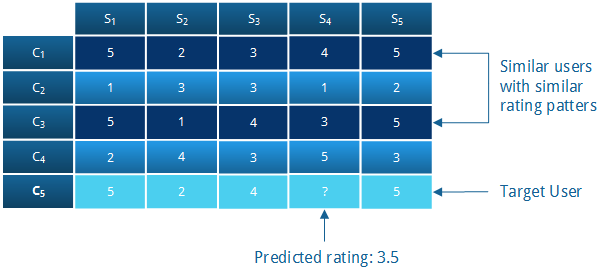
\includegraphics[scale=0.5]{image/ratingmatrix.png}
    \centering
    \caption[Collaborative filtering rating matrix]{Collaborative filtering rating matrix}
    \label{figure:ratingmatrix}
\end{figure}

Researchers have devised a number of collaborative filtering algorithms that
can be divided into two main categories: Memory-based and Model-based
algorithms \cite{Su2009}.

\begin{figure}[H]
    \centering
    \begin{tikzpicture}[
      rec/.style={
        rectangle,
        draw,
        text width=2cm,
        text centered
      },
      edge from parent fork down,
      level 1/.style={level distance=25mm,sibling distance=85mm},
      level 2/.style={level distance=25mm,sibling distance=25mm}
    ]
    \node[rec] {Collaborative filtering}
      child{
        node[rec] {Memory based}
        child { node[rec, align=center] {Item-based CF} }
        child { node[rec] {User-based CF} }
      }
      child{
        node[rec, align=center] {Model\\based}
        child { node[rec, align=center, right=-10mm] {Singular Value\\Decomp.} }
        child { node[rec, align=center] {Principal Component\\Analysis} }
        child { node[rec] {Baysian networks} }
        child { node[rec, align=center] {Rule-based\\stategies} }
        child { node[rec] {Clustering stategies} }
      }
    ;
    \end{tikzpicture}
    \caption[Classification of collaborative filtering techniques]{Classification of collaborative filtering techniques}
    \label{figure:cftaxonomy}
\end{figure}

\subsubsection{Memory-based Methods}
\marginpar{Change to Neighborhood models?}
\marginpar{Make clearer distinction between user-based and item-based}

Memory-based Collaborative Filtering methods utilize the entire user-item
database to generate predictions~\cite{Lin1994}. More formally, the value of an unknown
utility $u(c,s)$ for user $c$ and item $s$ is usually computed by taking the
weighted average of the utilities assigned by the $N$ most similar users for
the same item $s$. The similarity between user $c$ and $c'$, $sim(c, c')$ is
used as the weight. The more similar a user $c'$ is to $c$, the more weight is
given to the utility $u(c', s)$, and thus, will carry more weight in the
prediction for $u(c,s)$.

\begin{equation}
\label{equation:cfratingprediction}
u(c,s) = k * \sum_{c' \epsilon C} sim(c, c') * u(c',s)
\end{equation}

where k serves as a normalization factor, usually being $1/|C|$. Various
approaches have been used to compute the similarity $sim(c, c')$ between the
users. Generally these approaches are based on the rating similarities for
items both users have rated. The one of the most popular similarity measure is The Pearson
Correlation Coefficient. Equation \ref{equation:pearson} shows how to calculate
the Pearson Correlation Coefficient between two users $c$ and $c'$, Here
$S_{cc'}$ is the set of items both users have in \emph{common}.

\begin{equation}
sim(c, c') = \frac{\sum_{s \epsilon S_{cc'}} (u(c, s)-\bar{u_{c}})(u(c',s)-\bar{u_{c'}})}{\sqrt[•]{\sum_{s \epsilon S_{cc'}} (u(c, s)-\bar{u_{c}})^{2}(u(c',s)-\bar{u_{c'}})^{2}}}
\label{equation:pearson}
\end{equation}

where $u_{c}$ is the mean utility of user $c$. The Pearson Correlation
Coefficient and other similarity measures such as cosine based approaches are
more commonly known user-based collaborative filtering.

Item-based Top-N Recommendation methods calculates the similarity between items
instead of users. In these approaches, the historical information is analyzed
to identify the relations between items such that a purchase of another item
(or set of items) often leads to the purchase of another item. These models are
often used since they quickly can recommend a set of items, and have shown to
produce recommendation results comparable or better than traditional user-based
approaches \cite{Karypis2001}.

The algorithm first computes the $k$ most similar items for each item according
to the ratings given by users they both share. Once the most similar items are
found, the prediction is then computed by taking the weighted average of the
target user's ratings on these similar items.

\begin{equation}
u(c,s) = \frac{\sum_{all similar items, S} (sim(s,S)u(c, S)}{\sum_{all similar items, S}(|s,S|)}
\end{equation}

Items that often are rated similarly by users are considered more similar than
items which share few similar ratings. Figure \ref{figure:itemsim} illustrates
the process of finding the item-similarities.

\begin{figure}[H]
    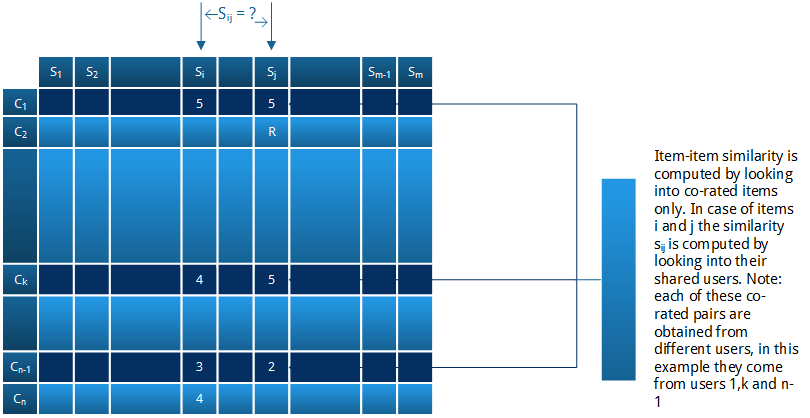
\includegraphics[width=5in]{image/itemsim.png}
    \centering
    \caption[Item-item similarity]{Item-item similarity}
    \label{figure:itemsim}
\end{figure}

There are a number of ways of computing the similarity between items, e.g. by
means of cosine-based similarity. In this case, two items are though of as two
vectors in an $C$ dimensional user space. The similarity between the items is
found by computing the cosine of the angle between the two vectors:

\begin{equation}
sim(s',s) = cos(\vec{s'},\vec{s}) = \frac{\vec{s'} \cdot \vec{s}}{\|\vec{s'}\|^{2} * \|\vec{s}\|^{2}}
\end{equation}

The item similarities can then used to find the Top-N recommendations. Each
user has a set of items $S_{c}$ previously rated by the user which we want to
compute top-N recommendations for. First, we identify the set $C$ of candidate
items recommendable by taking the union of the $k$ most similar items and
removing each of the items in the set $S_{c}$ the user already has rated; then
calculate the similarities between each item of the set $C$ and the set
$S_{c}$, using only the $k$ most similar items for each item in $S_{c}$. The
resulting set of items in $C$ are sorted in descending order of similarity and
will be the recommended as the item-based Top-N list \cite{Karypis2001}.
Items usually do not change as much as users, so this can often be computed offline.
Linden et al \cite{Linden2003} showed that item-based neighborhood methods also provide
another advantage over other methods, such as e.g. user-based neighborhood models:
in many industrial systems, most of the recommendation is made by the contextual
recommendation to anonymous users, as on the Amazon's website \marginpar{Add footnote}. This
recommendation is called item-to-item recommendation, and generally includes the archetype
associated message "people who have seen / bought this item also viewed / purchased these items.
This recommendation is directly based on an item-item similarity matrix on click or
purchase logs.

\subsubsection{Model-based Methods}
\label{model-based-methods}

As the name implies, Model-based approaches provide recommendations by first
developing a model of the user ratings, which is then used to make predictions~\cite{Su:2009:SCF:1592474.1722966}.
These algorithms develop a model of user ratings rather than identify a
neighborhood of similar users or items. These models can be built using various
strategies, such as Singular Value Decomposition (SVD), Principal Component
Analysis (PCA), Rule-based Strategies, Clustering Strategies and Bayesian
Networks.

Latent factor models is probably the most representative approach. Latent
factor models transform both items and users to a latent factor space. The
latent factor space tries to explain the ratings by characterizing both items
and users on factors automatically inferred from the data. The most popular
latent factor models are based on matrix factorization techniques
\cite{Koren2009}.

The main idea behind matrix factorization is just as its name implies,
factorize a matrix, finding two or more matrices such that when you multiply
them you get back the original matrix. Matrix factorization can be used to
discover latent factors underlying the interactions between the users and
items. These factors \emph{explain} how a user rates an item (i.e. that a user
would give high ratings to a certain shirt if he likes the brand, or if the
color is nice). If we can discover these factors, we should be able to predict
a rating with respect to a certain user and a certain item based on the
correlation between their factors.

A matrix factorization model map both users and items to a joint latent factor
space of dimensionality $f$, where $f$ is the number of latent factors. The
number of latent factors are usually determined by using a hold-out dataset or
cross-validation by evaluating the prediction error experimenting with
different values. It is also worth mentioning that this in some ways can be
seen as a trade-off between model building complexity and accuracy as having
more features makes the model building more expensive. Each user $c$ is
associated with a vector $p_{c} \epsilon \mathbb{R}^{f}$, and each item $s$ is
associated with a vector $q_{s} \epsilon \mathbb{R}^{f}$. Giving us a matrix Q
containing the user factors and a matrix P containing the item factors as
exemplified in Figure \ref{figure:matrixdecomp}.

\begin{figure}[H]
    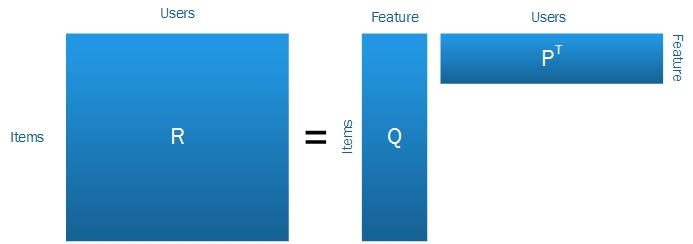
\includegraphics[width=5in]{image/matrixdecomp.jpg}
    \centering
    \caption[Matrix decomposition of the rating matrix $R$]{Matrix decomposition of the rating matrix $R$}
    \label{figure:matrixdecomp}
\end{figure}

User-item interactions are modeled as inner products in that space. For a given
item $s$, the elements of $q_{s}$ measures the extent to which the item
possesses those factors, positive or negative. Likewise, for a given user $c$,
the element $p_{c}$ measures the extent of interest that user has in items that
are high on the corresponding factors. The resulting dot product $\hat{u(c,s)}$
captures the overall interest of the user in the characteristics of the items.

\begin{equation}
u(c,s) = p_{c}^{T}q_{s} = \sum_{k=1}^{f} q_{sk}p_{kc}
\end{equation}

The problem then, is to discover the user factor matrix $P$ and the item factor
matrix $Q$ such that their product approximates the original rating matrix $R$.

\begin{equation}
R \approx Q \times P^{T} = \hat{R}
\label{equation:dotproduct}
\end{equation}

To learn the factor vectors the system minimizes the regularized square error
on the set of known rating $K$.

\begin{equation}
\label{equation:minimize}
min_{q, p} = \sum_{(c,s)\epsilon K} (u(c,s) - p^{T}_{c}q_{s})^{2} + \lambda ( \Vert q_{s} \Vert ^{2} + \Vert p_{c} \Vert ^{2})
\end{equation}

However, it is important to remember that our goal is generalize beyond the
observed ratings, in a way that we can predict future unknown ratings. The
system should therefore avoid overfitting the data by regularizing the learned
parameters, whose magnitudes are penalized. $\lambda$ controls the extent of
regularization, and much like $f$, often determined by cross-validation. Two
possible approaches to minimizing Equation \ref{equation:minimize} is to use
Stochastic Gradient Descent or Alternating Least Squares \citep{Koren2009}.\newline

Consider the following example where we have the following rating matrix R
shown in Table \ref{table:ratingMatrix} containing the rating of four users $C$
for four items $S$, giving us a $C \times S$ matrix with explicit ratings on a
  scale from 1 to 5.

\begin{figure}[H]
	\centering
	$
	\begin{bmatrix}
		5.00    & 5.00  & 2.00 & -    \\
		2.00    & -     & 3.00 & 5.00 \\
		-       & 5.00  & -    & 3.00 \\
		3.00    & -     & -    & 5.00
	\end{bmatrix}
	$
	\caption{Rating matrix $R$}
	\label{table:ratingMatrix}
\end{figure}

Given that $f = 3$, we might end up with the following matrix $P$ and $Q$

\begin{figure}[H]
\centering
$
\begin{bmatrix}
1.81    &1.62   &0.74\\
2.66    &1.71   &-1.08\\
1.73    &-0.23  &0.78\\
3.16    &-0.24  &0.90
\end{bmatrix}
$
\caption{User factor matrix $P$}
\end{figure}

\begin{figure}[H]
\centering
$
\begin{bmatrix}
1.12    &	1.49   &	0.48\\
1.31    &	-0.52  &	0.59\\
1.13    &	0.67	&	-0.52\\
1.39    &	0.05	&	0.45
\end{bmatrix}
$
\caption{Item factor matrix $Q$}
\end{figure}

Equation \ref{equation:dotproduct} then gives us the following rating prediction matrix $\hat{R}$.

\begin{figure}[H]
\centering
$
\begin{bmatrix}
4.79    &5.01   &1.97   &3.61 \\
1.97    &1.96   &2.85   &4.80 \\
2.75    &4.71   &1.40   &2.94 \\
2.93    &3.30   &2.74   &4.78
\end{bmatrix}
$
\caption{Rating prediction matrix $\hat{R}$}
\end{figure}



As you can see the values of known ratings in Table \ref{table:ratingMatrix}
are fairly similar to the corresponding ratings in the rating prediction
matrix.

\subsection{Hybrid approaches}

A term \emph{hybrid recommender systems} is used to describe any recommender
system that combines multiple recommendation techniques together to provide
recommendations. Burke et al. \cite{Burke2002} identified seven different
classes of hybrid recommender systems:

\begin{itemize}
\item Weighted: The score of different recommendation components are combined numerically.
\item Switching: Switching between recommender systems depending on the situation.
\item Mixed: Recommendations from different recommenders are presented together.
\item Feature Combination. Features derived from different knowledge sources
are combined together and given to a single recommendation algorithm
\item Feature Augmentation: One recommendation technique is used to compute a
feature or set of features, which is then part of the input to the next
technique.
\item Cascade: Recommenders are given strict priority, with the lower priority
ones breaking ties in the score of the higher ones
\item Meta-level: One recommendation technique is applied and produces some
sort of model, which is then the input by the next technique
\end{itemize}

Most commonly hybrid systems are built by combining collaborative and
content-based methods in an attempt to mitigate the limitations the approaches
suffer individually. Adomavicius and Tuzhilin \cite{Adomavicius2005} lists the
following approaches to building hybrid recommender systems:

\begin{itemize}
\item Implementing the systems separately and combining their predictions
\item Incorporating content-based characteristics into a collaborative approach
\item Incorporating collaborative characteristics into a content-based approach
\item Constructing a general unifying model that incorporates both
content-based and collaborative characteristics
\end{itemize}

\marginpar{heri-notes: Which approach relevant to this work?}

\subsection{Recommender System Challenges}

Below we briefly mention some of the main challenges one faces when working
with recommender systems.

\subsubsection{Scalability}

As the number of existing users and items blow up, traditional CF algorithms
suffer serious scalability problems. The model building phase of \emph{Traditional}
collaborative filtering methods have a complexity of O(MN) where $M$ is the number
of users and $N$ is the number of items. For systems with millions of users and items,
even a complexity of $n$ is too large. Another fundamental issue is how to embed the
core recommendation techniques in real operational systems and how to deal with massive
and dynamic sets of data produced by the interactions of users with items. Recommender
systems are expected in many cases to provide rapid recommendations online, it is
therefore also important to consider how fast the system provides recommendations.

Better scalability and improved accuracy make the item-item collaborative filtering
approaches more favourable in many cases. The computational complexity of item-to-item
based algorithms are up to two orders of magnitude faster than traditional user-based
algorithms \cite{Deshpande2004}. Dimensionality reduction techniques such as
SVD can deal with the scalability by providing more compact representations and
quickly produce good recommendations. However, most dimensionality reduction
techniques must undergo expensive matrix factorization steps.

\subsubsection{Sparsity}

In practice, many recommender systems deal with very large item collections.
This means that the number of ratings obtained is usually very small compared to the
number of ratings that it needs to predict. Efficient prediction of ratings from a small
number of examples is therefore important. The \emph{reduced coverage} problem
occurs when the number of users' rating may be very small compared to the number of items.
This may lead to that the recommender is unable to provide recommendations for a large
portion of the items. \emph{Neighbour transitivity} refers to the problem in which users
with similar tastes may not be identified due to a lack of co-rated items, making
collaborative filtering futile, since it relies on comparing users to predict unknown ratings.

\subsubsection{Cold-start}

Conceptually, the cold-start problem can be viewed as a special instance of the
sparsity problem, where most elements in a certain row or column are zero. The
cold-start problem further emphasizes the importance of the sparsity problem.
Whenever a new user or item enters the system, it is difficult to find similar
ones as there is little or no information available. New items can therefore
not be recommended until they have been recommended by a substantial amount of
users. Similarly, giving \emph{good} personalized recommendations to new users
based on a few ratings is difficult, since it does not give a good overall
picture of a users tastes and preferences. These problems are known as the
\emph{cold-start user} and \emph{cold-start item} problems.

\subsubsection{Shilling attacks}

In recommender systems where everyone can give ratings, people may give lots of
positive ratings to their own items and negative ratings to their competitors.
It is often necessary for collaborative filtering systems to introduce
precautions to discourage such kind of manipulation.

\subsection{Terminology}

\marginpar{TODO: Fjerne?}

%TODO - Any more RS related terminology that needs explaining?

\subsubsection{Explanations / Transparency}

\marginpar{heri-notes: Hvorfor har dere med dette?}

Tintarev et al. \cite{Tintarev2007} lists seven roles a that can be played by explanations in recommender systems:

\begin{itemize}
\item Transparency: Explaining how the system works
\item Scrutability: Allowing the users to tell the system it is wrong
\item Trust: Increasing user confidence in the system
\item Effectiveness: Help users make good decisions
\item Persuasiveness: Convince users to try or buy
\item Efficiency: Helping users to make decisions faster
\item Satisfaction: Increasing the ease of use or enjoyment
\end{itemize}

In collaborative filtering systems the explanations is of the form "Other users
similar to you liked this item", while in content-based style explanations, the
item's attributes which most affected the item to be recommended to the user
are illustrated. For example, in a fashion recommender, an explanation may be
of the form "This shirt was recommended because it's a Ralph Lauren who you
seem to like".

% !TEX root = ../../report.tex

\section{Fashion Recommendation}

\subsection{Fashion theory}
\label{subsec:fashion-theory}

Our first goal (\textbf{Goal G1}) is to better understand the fashion domain.
To achieve this a detailed study is needed, both to better understand
\textit{how} we want to predict user preferences, but also to explain various
effects seen in the dataset. We first study the broad definition of
\textit{fashion} and what its implications are on consumer behavior. Next we
study how the fashion industry is experiencing tremendous growth in the
e-commerce sector, before finally looking at the SoBazaar application --
performing a comprehensive competitor analysis where we try to identify the
largest segments of both growth potential and recommendation system
uniqueness.

\subsubsection{Definition}

There exists multiple interpretations and different definitions of the term
\textit{fashion}. However, by looking at a set of definitions we can observe a
common theme.

\begin{itemize}
    \item \textit{The entire spectrum of attractive clothes styles at any given
    time} - Anne Hollander

    \item \textit{Fashion is dress in which the key feature is rapid and continual
    changing of styles} - Elisabeth Wilson

    \item \textit{Fashion is usually first raised by a small group of people
    and then a trend is formed with more and more followers and copycats till
    it becomes outdated} - Cheng \& Huang

    \item \textit{The social norm recognized and advocated by a particular
    social class at one time. It affects all the fields in society, especially
    and famously in clothing. Sometimes, short-lived fashion is referred to as
    style} - Fang Ma \cite{Fang2012}

\end{itemize}

The recurring themes can be classified as being related to clothes, popularity,
time and cultural grouping. One of the main drives of fashion is the need and
want for belonging, and for individuals to become a part of something bigger
-- sharing a common thought or opinion. A common term to use is \textit{making a
fashion statement}, where a group or individual makes their opinion or
statement heard without words, but through clothing and fashion. When making
recommendations this is important, as social connections between users become
important and can potentially be used to enhance predictions and understand
subcultures within communities. In addition we notice that \textit{per
definition} recentness and popularity are two important factors to fashion,
hence this should be reflected in both understanding implicit feedback and
making recommendations.

So fashion is what a \textbf{social group}, or a \textbf{set of groups},
recognizes and highly advocates \textbf{at any one time}. Thus in broader
terms we can classify music, hair and many other trends as being fashion as
well -- however, when referencing the term \textit{fashion} in this thesis we
implicitly refer to clothing and accessories.

Hanf et. al.~\cite{Hanf1994} states that customers are rational, when it comes
to price and quality. This if further verified by~\cite{dutton2006} where the
attributes classified as making the largest impact on customers are styling,
brand, price, store (physical location) and fabrication/quality. The complete
list of attributes and their relations is shown in
Table~\ref{table:ConsumersPurchaseDec}. These attributes are important to take
note of, as they will become important features in both training and predicting
recommendations.

Culture is one of the main factors to determine consumer behavior.  Culture can
be segmented into two parts: subculture and social class. All consumers are
included in many smaller subcultures such as nationality, religious subcultures
and geographical subcultures. The forming of a subculture happens through
individuals seeking out other individuals with similar tastes regarding a
variety of aspects.~\cite{vignali2009fashion}. With a larger dataset than what
is currently is available in SoBazaar one should be able to automatically
classify subcultures and social classes based on buying behavior, brands,
price and popularity scores and demographics.

Finally, we note that the brand of the product might also greatly affect what
the consumer buys and what the consumer does not buy. A study done on the
behavior of the consumer~\cite{deLace2010} showed that knowing the brand of two
almost identical products made the consumer crowd shift towards the more well
known brand. In comparison, when the users did not know the actual brands of
the products, they yielded an almost equal distribution on the products. In
SoBazaar, as in the fashion domain in general, there is consequently a large
focus on brands. However, when recommending novelty is a key figure -- that is
we want to introduce users to \textit{new} products as well as brands.

\subsection{Recommendation challenges}
\label{subsec:rec-challenges}

There are many challenges when making recommendations in the fashion domain,
especially compared to other domains. In this subsection we will take a look at
some challenges already mentioned as well as introduce a brief discussion on
how one might go about and solve them in a recommender system.  This is done in
order to fulfill our second research goal (\textbf{Goal G2}) and to lay the
foundations upon which we conduct further research and implementations.

\paragraph{Recentness and seasons}
As seen, time is \textit{per definition} a central feature in fashion, and
consequently an important aspect to consider when analyzing implicit feedback
and making recommendations. There are many types of recentness to consider:

\begin{itemize}
\item Apparel may go out of season.
\item Or go \textit{out of fashion}, that is experiencing a lowered popularity.
\item Or be replaced by newer collection.
\item Users tastes may change, due to a range of external factors.
\end{itemize}

In a recommender system we need to account for these factors by finding some
way of penalizing old items combined with low popularity. Further, different
from other domains, we need to expire feedback given from the user after a
fixed time interval as we assume the tastes changes over time.

\paragraph{Implicit data}
The feedback from the user will mainly be implicit~\ref{sec:implicit}, and if
the users had the possibility of rating an item there is no way of knowing
\textit{which} features contributed to a positive rating -- without much data.
Instead we assume that an increased interest in an item is correlated with
increased interaction with the item, an hypothesis that per~\ref{sec:conv-rate}
and Table~\ref{tab:prob-purchase} holds true, as we see more visits on an item
increase the probability of purchases. As seen per definition users are also
highly price and brand-aware and hence we should utilize this information in a
future recommender system, trying to classify users by their preferences in
terms of product features.

\paragraph{Product semantics}
In SoBazaar we aggregate products from a variety of different webstores into a
single product database. From each store we extract products that all contains
features such as color, type, target group, style and others - however the
quality of this input is diverse and in some scenarios much of the data is
lacking. This is a common issue in content based recommending, where we need to
convert our product descriptions and semantics into \textit{structured} data.
This can be done by various natural language processing techniques, where
challenges are both ambiguity, sparsity and language detection. An example is
trying to define, based on product semantics, whether a blouse is conservative
or flashy? How trendy is it? Is it casual or formal? And so
forth.~\cite{ghani2002building}

\paragraph{Novelty and coverage}
Some recommender systems produce highly accurate recommendations, with
reasonable coverage, but which are ineffective for practical purposes. For
instance, we may recommend an highly popular item to all users that everyone
has a pre-existing knowledge of, but given this knowledge still chose to not
interact with the product. Instead we should aim for recommending items that
both scores well, but that the user has never seen before. This property is
called increasing the \textit{novelty} of recommendations and are important in
the fashion domain, and as we can see closely related to recentness, as we wish
to introduce users to \textit{new} items and give them inspiration for new
styles. The \textit{serendipity} is increased when we in addition recommend
items that positively surprises the user, and which the user would not have
found given usual shopping patterns. Hence we would like to not only recommend
based on brands and clothes the users most often frequent, but enhance the
experience by including untraditional choices.

\paragraph{Fluctuating prices}
As seen in the previous section, price is an important factor when considering
both fashion marketing and user behavior. Users are browsing through multiple
sites in order to find the best offer, and research is an important part of the
shopping experience. Price should also be presented to the user when they have
the possibility to interact with it, so that we can assure ourselves that all
actions (e.g. wanting a product) are done knowing the retail price. Prices in
the fashion domain are also highly fluctuating and this can be taken advantage
of in a recommender system by presenting good deals to the user and informing
about upcoming sales on items which they might find interesting. It can also
help retailers target their sales campaigns towards items with high activity,
but low conversion.

\paragraph{Demographics, subcultures and social-classes}
Demographics and the social aspect in fashion is very important and can be
utilized in a recommender system by looking at user properties such as
location, friends, occupation, sex, age and, in the case of a social network
such as Facebook, their liked Pages exposing which interests the user may have.


\subsection{E-commerce and the fashion industry}
\label{sec:fashionInEcom}

The term \textit{e-commerce} is used when referencing businesses trading
services and products via the internet. There are many different types of both
services and products traded - but considered both largest and fastest growing
is trading goods in the fashion industry. In the UK the online sector of
fashion has grown 258\% in five years, yielding a yearly growth of almost
29\%~\cite{Divante2014}.

As seen in Figure~\ref{fig:ecommerce-norway} the same growth can be observed in
Norway, where purchases in the e-commerce industry has had a steady increase
since 2005 - although no specific numbers on the fashion industry alone are
available.

This large segment of e-commerce has many unique properties not found in other
domains, but of which the reader should be aware of - as they greatly affect
both which features and properties we can look at for making recommendations
and they form an important backbone for understanding the SoBazaar dataset.
We introduce this section by looking at one of the areas where the fashion
domain really stands out -- an area where an important property about SoBazaar
target group can be observed.

\begin{figure}[H]
    \centering
    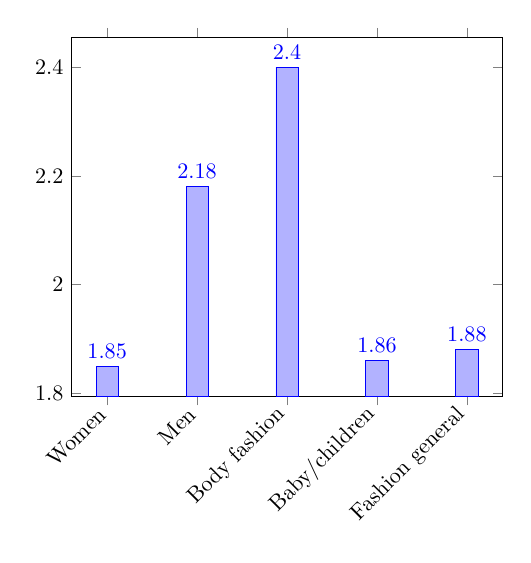
\begin{tikzpicture}[scale=0.8]
      \begin{axis}[
        ybar,
        symbolic x coords={Women, Men, Body fashion, Baby/children, Fashion general},
        x tick label style={rotate=45, anchor=east},
      ]
      \addplot +[nodes near coords] coordinates {
        (Women, 1.85)
        (Men, 2.18)
        (Body fashion, 2.40)
        (Baby/children, 1.86)
        (Fashion general, 1.88)
      };
      \end{axis}
    \end{tikzpicture}
    \caption{Conversion rate in various fashion segments}
    \label{fig:conversionRateFashion}
\end{figure}

This figure is taken from~\cite{Jorij2012} and shows the conversion rate for
various segments in the fashion domain. The conversion rate is the portion of
users who visits a website, and reaches the target (makes a conversion) set
by the site. For most e-commerce application, a conversion
is counted when a purchase is made. The conversion rate $r$ can easily be
calculated by $r = \frac{|Conversions|}{|Total visits|}$~\cite{nielsen2013}.
We can see that womens has the lowest conversion rate among the different
segments, indicating that there is a strong preference based shopping
tendency and that many users are \textit{browsing} and searching for the
right product. This hypothesis is strengthen by looking at the general
conversion rate in the e-commerce industry, which lies at 3\%. The potential
of a personalized recommender could in other words make browsing easier and
hence increase the conversion rate.

When making a purchase in the SoBazaar application, the user is redirected to the retailer selling the item, so the purchase is not done in the application.
This can lead to a higher \emph{purchase count} than the actual truth, but is what can be considered the conversion in the SoBazaar application.
For SoBazaar there are 18200 sessions in total and 1488 purchases, so the conversion rate is $0.08175824175 = \frac{1488}{18200}$, which is quite high compared to the conversion rate in women fashion from figure~\ref{fig:conversionRateFashion}, which was expected, since it is no commitment to making a purchase in the SoBazaar application.

\begin{figure}[H]
  \begin{tabular}{cc}
    \resizebox{0.43\linewidth}{!}{
      \begin{tikzpicture}
        \pie[text=legend, rotate=60]{
          34.30/Women,
          13.43/Men,
          17.91/Generalist,
          11.94/Body,
          4.47/Shoes,
          2.98/Jeans,
          14.97/Other
        }
      \end{tikzpicture}
    }
    \resizebox{0.49\linewidth}{!}{
      \begin{tikzpicture}
        \pie[text=legend, rotate=60]{
          15/Direct,
          23/Paid,
          30/Organic,
          5/CPS,
          9/CPC,
          8/Viral or social,
          10/E-mail newsletter
        }
      \end{tikzpicture}
    }
  \end{tabular}
  \caption{Distribution of target groups and traffic sources in the fashion
  domain}
\end{figure}

Both figures are adopted from~\cite{Jorij2012}, basing its results from a study
with 70 participating fashion companies with the goal of doing a complete
benchmark of the industry. In the leftmost figure we see how the different
e-commerce fashion retailers focuses their products. We observe that a large
majority of e-commerce fashion companies are targeting women - as is
SoBazaar.  Underlining the compensative market and the need to stand out to
the customer, by e.g. having personalized recommendations.

In the rightmost figure it is shown from where the customers originate in
online retails stores. The \textit{Paid} and \textit{Organic} are synonymous
with a user entering the site via. research or ads in the search engine, and
stands for 53\% of the traffic in e-commerce fashion - highlighting the
importance of a good reputation and digital profile. Direct traffic is as low
as 15\%, compared to the e-commerce industry in general where the same number
is 22.3\% \cite{Jorij2012}. This is explained by non-fashion products often
being offered in multiple stores and the users are thus browsing multiple sites
to find the best offer. Lastly we note that the viral/social segment is rather
small at 8\%, but compared to the e-commerce industry in general at 4\%. Hence
we conclude that although a small set of users interact with fashion companies
by social media, it is still a more important segment for this industry
compared to the e-commerce industry in general.

\subsection{Competitor Analysis}
\label{subsec:competitors}

As seen in the previous section, SoBazaar is not the only e-commerce
application in the fashion domain, with multiple competitors, and constantly new competitors entering the scene. Nor is it the first of its kind.

In this section some of these competitors will be explored,
looking into their strengths, weaknesses and features in regards to providing
recommendations for the user. This is both to better understand the fashion
domain (\textbf{Goal G1}) and to study existing technologies and how they are
applied (\textbf{Goal G3}). Using this data we can analyze the potential of
SoBazaar in e-commerce market, in addition we can understand both how users are
used to interact with similar applications and where we should focus in order
to enhance the uniqueness of the solution, creating a competitive advantage.

\subsubsection{Myntra}
\label{par:myntra}

"Myntra.com is a one stop shop for all your fashion and lifestyle needs" -
about Myntra~\cite{myntra}.

Myntra is one of India's largest e-commerce stores for fashion and aims to
provide a hassle free shopping experience for the user.  They aim to bring the
newest and most in-season fashion products available to the user trough the web
store front.  The brand base of Myntra consists of 500 leading brands from both
inside and outside India.

The web page uses a set of recommendation approaches to inform the user of what
they might like, and to increase the user's awareness of different kinds of
items. Such as, similar item and most popular. In this figure we can see in red
how Myntra is suggesting items which are similar to the item the user is
currently looking at

\begin{figure}[H]
    \centering
    \fbox{
      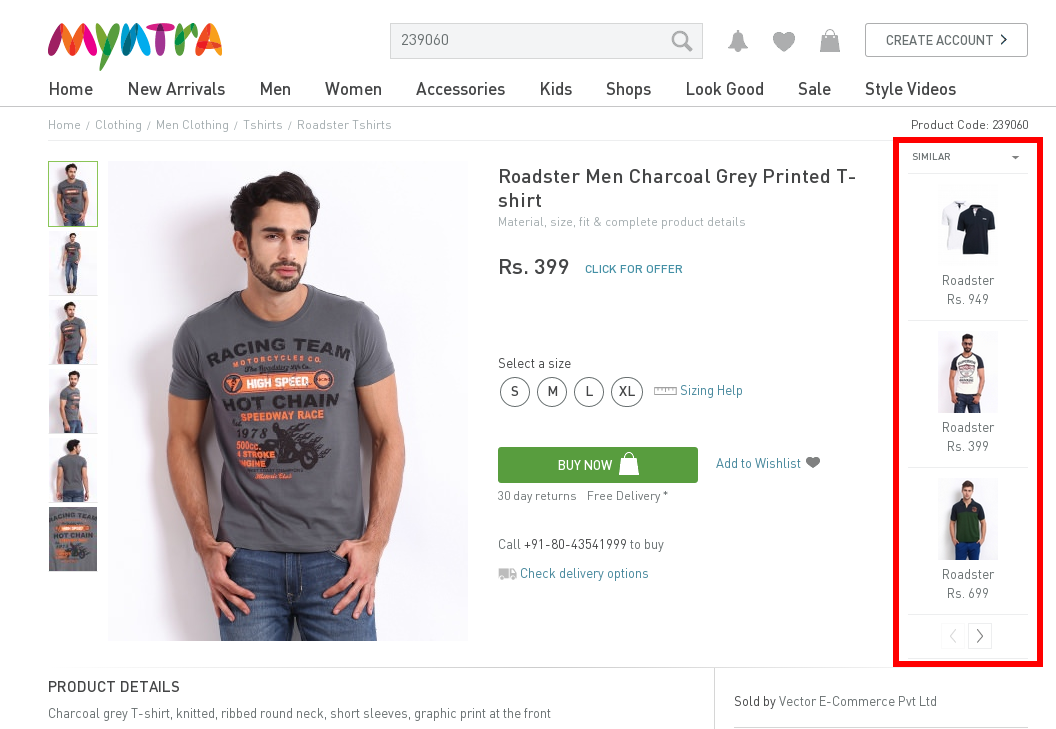
\includegraphics[scale=0.4]{image/myntiaSimilarExample.png}
    }
    \caption[Example of Myntra's "similar item" approach]{Example of Myntra's
    "similar item" approach}
    \label{figure:myntiaSimilarEx}
\end{figure}

This table is the list of the recommendation related strengths and weaknesses
of the e-commerce fashion web site Myntra~\cite{myntra}

\begin{table}[H]
    \centering
    \begin{tabularx}{\linewidth}{>{\parskip1ex}X@{\kern4\tabcolsep}>{\parskip1ex}X}
        \toprule
        \hfil\bfseries Strengths
        &
        \hfil\bfseries Weaknesses
        \\\cmidrule(r{3\tabcolsep}){1-1}\cmidrule(l{-\tabcolsep}){2-2}
        %Strengths
        Suggest similar items connected to the currently viewed \par
        Popular list for the different brands and stores \par
        Ability to add item to a "want list"\par
        &
        %Weaknesses
        No personalized recommendations \par
        \\\bottomrule
    \end{tabularx}
    \caption{Myntra: Strengths and weaknesses}
    \label{table:ecommerceMyntra}
\end{table}

\subsubsection{Asos}
\label{par:Asos}

"ASOS is a global online fashion and beauty retailer selling over 65,000 branded and own-label products" -
about Asos~\cite{asos}.

Asos have more than 29 million unique visitors per month and ship to more than 234 countries and territories.

The web page gives the user the ability to add products directly to a shopping chart.
When accessing an item, the user is presented with a set of items which asos recommends for the user.
They also present a set of clothes which might \emph{complete the look}, these recommendations are products which are assumed to \emph{go well} with the current item.
The users can also like and save items for later.
Other features are \emph{most popular} and \emph{outfits \& looks}.
\emph{Outfits \& looks} is a community where the user is given a set of options, amongst them are; voting for items, shop looks, gather \emph{style credits} and follow other users.

This table is the list of the recommendation related strengths and weaknesses
of the e-commerce fashion web site Asos~\cite{asos}

\begin{table}[H]
    \centering
    \begin{tabularx}{\linewidth}{>{\parskip1ex}X@{\kern4\tabcolsep}>{\parskip1ex}X}
        \toprule
        \hfil\bfseries Strengths
        &
        \hfil\bfseries Weaknesses
        \\\cmidrule(r{3\tabcolsep}){1-1}\cmidrule(l{-\tabcolsep}){2-2}
        %Strengths
        Suggest similar items connected to the currently viewed \par
        Popular list for the different brands and stores \par
        Ability to add item to a "want list" \par
        Suggest items which might \emph{go well} with other items \par
        Follow other users \par
        &
        %Weaknesses
        No personalized recommendations \par
        \\\bottomrule
    \end{tabularx}
    \caption{Asos: Strengths and weaknesses}
    \label{table:ecommerceAsos}
\end{table}


\subsubsection{Mallzee}
\label{par:Mallzee}

"Say hello to Mallzee, your nifty, personalised shopping app with a social twist. Instantly purchase, save for later or ask your nearest and dearest for their opinion on your latest fashion discovery." - about Mallzee~\cite{mallzee}.

Mallzee is a mobile phone application intended to ease shopping trough gathering fashion stores in one place, and have more than 2 million products from over 100 stores.

The applications utilizes a \emph{hot-or-not} approach, where the user can like or dislike products, this feedback is used to recommend other products the user might like.
Users can also get feedback from other users.

This table is the list of the recommendation related strengths and weaknesses
of the e-commerce fashion mobile application Mallzee~\cite{mallzee}

% \begin{table}[H]
%     \centering
%     \begin{tabularx}{\linewidth}{>{\parskip1ex}X@{\kern4\tabcolsep}>{\parskip1ex}X}
%         \toprule
%         \hfil\bfseries Strengths
%         &
%         \hfil\bfseries Weaknesses
%         \\\cmidrule(r{3\tabcolsep}){1-1}\cmidrule(l{-\tabcolsep}){2-2}
%         %Strengths
%         Presented with what friends like \pars
%         Ability to add item to a "want list" \par
%         Follow other users \par
%         Hot-or-Not approach \par
%         Personalized recommendations \par
%         &
%         %Weaknesses
%         No most popular list \par
%         Redirected on purchase \par
%         \\\bottomrule
%     \end{tabularx}
%     \caption{Mallzee: Strengths and weaknesses}
%     \label{table:ecommerceMallzees}
% \end{table}


\begin{table}[H]
    \centering
    \begin{tabularx}{\linewidth}{>{\parskip1ex}X@{\kern4\tabcolsep}>{\parskip1ex}X}
        \toprule
        \hfil\bfseries Strengths
        &
        \hfil\bfseries Weaknesses
        \\\cmidrule(r{3\tabcolsep}){1-1}\cmidrule(l{-\tabcolsep}){2-2}
        %Strengths
        Suggest similar items connected to the currently viewed \par
        Popular list for the different brands and stores \par
        Ability to add item to a "want list" \par
        Suggest items which might \emph{go well} with other items \par
        Follow other users \par
        &
        %Weaknesses
        No personalized recommendations \par
        \\\bottomrule
    \end{tabularx}
    \caption{Asos: Strengths and weaknesses}
    \label{table:ecommerceMallzees}
\end{table}

\subsubsection{Lyst} % (fold)
\label{par:lyst}

"Lyst.com is a fashion shopping site that gives you your own shopping
experience, so you can discover more of the fashion you love" - About
Lyst~\cite{lyst}.

Lyst offers items from thousands of the leading brands and stores of the world.

The site allows the user to follow different stores or brands to receive the
latest items they have to offer.  The user is given a personalized "stylefeed",
which displays items from the different brands or stores the user is following.
It is also possible for the user to add items to the their profile.

On first login the user is presented with a set of brands and store the user
can like or dislike, to get the "stylefeed" started.  On access of an item, the
user is presented with related items, and the ability to add the item to a
collection.  When the user wants to buy an item, the site will redirect the
user to the store selling the item.

\begin{table}[H]
  \centering
    \begin{tabularx}{\linewidth}{>{\parskip1ex}X@{\kern4\tabcolsep}>{\parskip1ex}X}
    \toprule
      \hfil\bfseries Strengths
        &
        \hfil\bfseries Weaknesses
        \\\cmidrule(r{3\tabcolsep}){1-1}\cmidrule(l{-\tabcolsep}){2-2}
                Can follow brands and stores \par
                Connected with facebook \par
                Ability to add item to a "want list" \par
                "Stylfeed" based the user's follow list \par
                Show related items \par
                &
                Limited personalized recommendations \par
                \\\bottomrule
            \end{tabularx}
    \caption[Recommendation related strengths and weaknesses of Lyst~\cite{lyst}]{This table is the list of the recommendation related strengths and weaknesses of e-commerce fashion web site Lyst~\cite{lyst}}
    \label{table:ecommenreceLyst}
\end{table}

\subsubsection{Farfetch} % (fold)
\label{par:farfetch}

"farfetch.com forms the hub of a global fashion community that unites
independent boutiques around the world with fashion lovers" - About
Farfetch~\cite{Farfetch}

Farfetch is a collection of over 1000 boutiques from all over the world
gathered on one web page.  The user can shop directly on the page, and get the
item delivered to the doorstep with only one checkout process.

When browsing an item the user is presented with a set of recommendations
related to the current item, and previous browsing history.  The item can be
added to a "want list" or to the shopping chart.

\begin{figure}[H]
    \centering
    \fbox{
      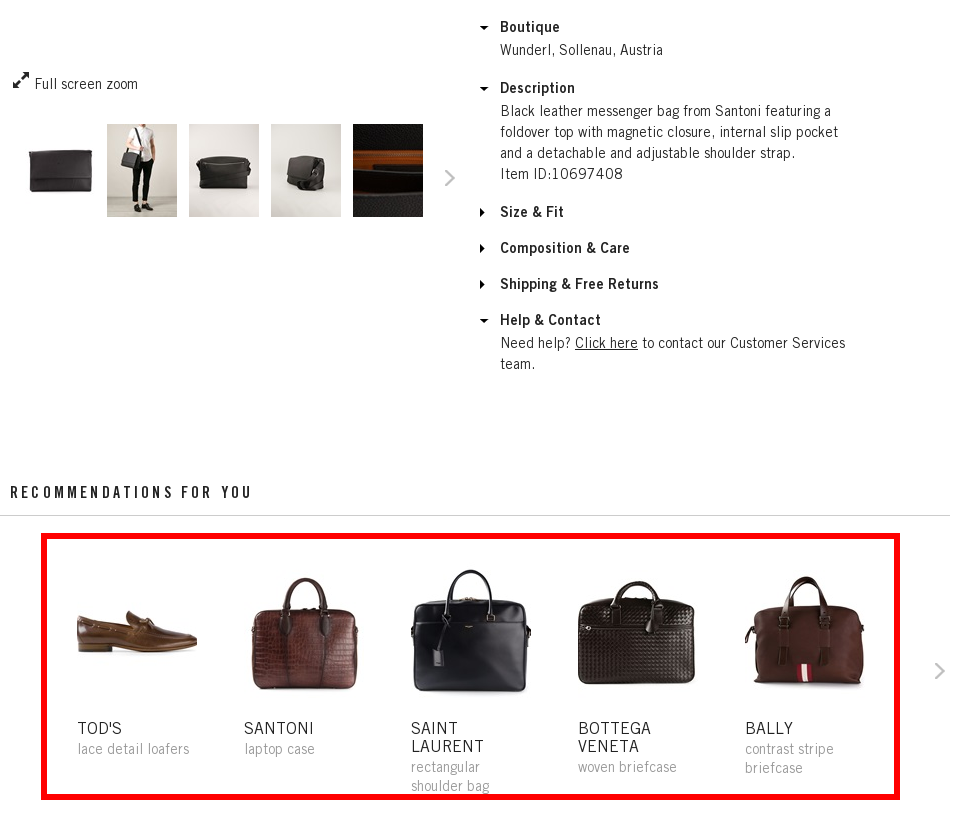
\includegraphics[scale=0.4]{image/farfetchedRecommendationExample.png}
    }
    \caption{Example of Farfetch's recommendations}
    \label{figure:farfetchedRecommendationExample}
\end{figure}

In this figure we can see in red how Farfetch is recommending items which might
be of interest to the user. As we can see the first item is a shoe, which was
the last item accessed by the user, the next four items are related to the
currently viewed item.

\begin{table}[H]
    \centering
    \begin{tabularx}{\linewidth}{>{\parskip1ex}X@{\kern4\tabcolsep}>{\parskip1ex}X}
      \toprule
      \hfil\bfseries Strengths
      &
      \hfil\bfseries Weaknesses
        \\\cmidrule(r{3\tabcolsep}){1-1}\cmidrule(l{-\tabcolsep}){2-2}
        %Strengths
            Ability to add item to a "want list" \par
            A feed with the most popular items \par
            A feed with new items \par
            A list of recommendations for the user \par
          &
          %Weaknesses
            No option to follow other users \par
         \\\bottomrule
    \end{tabularx}
    \caption[Recommendation related strengths and weaknesses of Farfetch~\cite{Farfetch}]{This table is the list of the recommendation related strengths and weaknesses of e-commerce fashion web site Farfetch~\cite{Farfetch}}
    \label{table:ecommenreceFarfetch}
\end{table}

\subsubsection{MyHabit}
\label{par:myhabit}

"MyHabit is a private fashion sale site offering up to 60\% off hand-picked
selections from designer and boutique brands." - About MyHabit~\cite{MyHabit}

MyHabit was founded by Amazon in response to the desire from the users of
Amazon to shop fashion in an easy manner.

The site displays a feed.  This feed is fed by a team from MyHabit, and is
constantly updating with new sales and new products.  The items put into the
feed are handpicked.

When browsing items on MyHabit, other similar items are suggested to the user.

\begin{table}[H]
  \centering
  \begin{tabularx}{\linewidth}{>{\parskip1ex}X@{\kern4\tabcolsep}>{\parskip1ex}X}
    \toprule
    \hfil\bfseries Strengths & \hfil\bfseries Weaknesses \\
    \cmidrule(r{3\tabcolsep}){1-1}\cmidrule(l{-\tabcolsep}){2-2}
    Shop on site \par
    Similar items \par
    &
    No personalized recommendations \par \\
    \bottomrule
  \end{tabularx}
  \caption[Recommendation related strengths and weaknesses of MyHabit~\cite{MyHabit}]{This table is the list of the recommendation related strengths and weaknesses of e-commerce fashion web site MyHabit~\cite{MyHabit}}
  \label{table:ecommenreceMyHabit}
\end{table}

\subsubsection{Competitors Recommendation Overview}
\label{par:competitors_recommendation_overview}

In table~\ref{table:ecommerceCommpetiros} we see that there is a very low count
of fashion related e-commerce applications, which actually produces
personalized recommendations for their users.

Most of applications are taking a simpler approach when making recommendations
for the user, like most popular or similar items.  There is no obvious relation
between recommendations and that the site has a form of "want list", but the
system which allows the users to follow each other are usually not
in-application-purchase-applications.

There where no indications of the "want list" being used directly to some
personalized recommendations and neither was it any indication that the "follow
list" of other users helped produce any personalized recommendations, other
than recommending items from the followed user's feed.  The "follow list" was
also in some cases used to suggest other users to follow.  The "want list" was
primarily there so that the user could go back to a liked item, and maybe
interact with it later.

\begin{table}[H]
    \centering
    \begin{tabular}{l l l l l l l}
        \toprule
        Competitor &
        \multicolumn{1}{l}{\parbox{1.3cm}{ In App \\ Purchase}} &
        \multicolumn{1}{l}{\parbox{1.0cm}{ Most \\ Popular}} &
        \multicolumn{1}{l}{\parbox{1.0cm}{ Similar \\ Items}} &
        \multicolumn{1}{l}{\parbox{1.0cm}{ Want \\ List}} &
        \multicolumn{1}{l}{\parbox{1.9cm}{ Follow \\ Other Users}} &
        \multicolumn{1}{l}{\parbox{2.6cm}{ Personalized \\ Recommendations}} \\ \midrule

        Myntra  & \cmark & \cmark & \cmark & \cmark & \xmark & \xmark \\
        Flink   & \xmark & \cmark & \cmark & \cmark & \cmark & \xmark \\
        Lyst    & \xmark & \cmark & \cmark & \cmark & \cmark & \xmark \\
        Motilo  & \xmark & \cmark & \xmark & \cmark & \cmark & \xmark \\
        Farfetch & \cmark & \cmark & \cmark & \cmark & \xmark & \xmark/\cmark~\tablefootnote{How the recommendations are produced is not mentioned} \\
        ModCloth  & \cmark & \cmark & \cmark & \cmark & \xmark & \xmark \\
        UsTrendy  & \cmark & \cmark & \cmark & \cmark & \xmark & \xmark \\
        Polyvore  & \xmark & \cmark & \cmark & \cmark & \cmark & \xmark \\
        Clothia  & \xmark & \cmark & \cmark & \cmark & \cmark & \xmark \\
        Trendabl  & \cmark & \cmark & \cmark & \cmark & \cmark & \xmark \\
        Zalando  & \cmark & \cmark & \cmark & \cmark & \xmark & \xmark \\
        Ellos  & \cmark & \cmark & \cmark & \cmark & \xmark & \xmark \\
        LookBook  & \xmark & \cmark & \cmark & \cmark & \cmark & \xmark \\
        Fahsiolista  & \xmark & \cmark & \xmark & \cmark & \cmark & \xmark \\
        ShopStyle  & \xmark & \xmark & \cmark & \cmark & \xmark & \xmark \\
        MyHabit  & \cmark & \xmark & \cmark & \xmark & \xmark & \xmark \\
        Asos  & \cmark & \cmark & \cmark & \cmark & \cmark & \xmark \\
        Mallzee  & \xmark & \xmark & \xmark & \cmark & \cmark & \cmark \\
        Kwoller  & \xmark & \xmark & \xmark & \cmark & \xmark & \cmark \\
        \bottomrule
    \end{tabular}
    \caption{Properties of different e-commerce application}
    \label{table:ecommerceCommpetiros}
\end{table}

Show in the table~\ref{table:ecommerceCommpetiros} above is the list of the
different properties of some of the different competitors to SoBazaar. The
properties are in regards of their recommendation ability, and how they let
their user expand their item set A more complete list can be found in the
appendix~\ref{app:sec:soCompetitors}.

\subsection{Fashion Recommender Systems}

This subsection will look at different methods other fashion related
systems have used to recommend fashion related products to the user.

\subsubsection{Photograph based approach}
    Fashion and the products it regards are highly dependent on visuals.  A fashion
    product would not be very interesting if no one saw it.  An approach to use the
    importance of how the product looks regarding recommending is to utilize images
    of the product.  Fashion Coordinates Recommender System Using Photographs from
    Fashion Magazines~\cite{Iwata:2011} is a system doing this.  They teach their
    system by using fashion magazines with full body images.  They segment the
    image into two parts, top and bottom.  From this the system learns which top
    matches to which bottom and collects visual features of the products.  From
    this the system can recommend other tops to go with a selected bottom, or other
    way around.  The proposed system scored better\footnote{Accuracy of 50\% on the
    top 5 suggested items, whereas naive and random managed 18\% and under 5\%
    respectively} than both a more naive approach and a random selection.  Runtime
    was at 0.04 seconds per recommendation.

\subsubsection{Hot-or-not}
    A recommender system called SuitUp~\cite{SuitUp} did a survey on some of their potential users.
    One interesting finding was that many of the users enjoyed the Hot-or-Not feature of the system.
    This feature gives the user a set of items and the option to either like or dislike.
    This did not only make the participants in the survey more engaged in the system, but also produced ratings, both negative and positive, for the system.
    For cold-start users and in a cold-start system this extra information and ratings make it much easier to make recommendations for the users.

\subsubsection{Scenario-Oriented Recommendation}
    Shen et al.~\cite{Shen:2007:AIG:1216295.1216368} proposed a recommender system which produce recommendations not only based on the metadata of the products, but also on user written input.
    Knowledge used to handle the user input, is derived from Open Mind Common Sense~\cite{Singh02openmind}.

    The user uploads his or her clothes and adds brand (e.g.Nike), type (e.g.jeans), material and a description about the item (e.g."I put these on when I get home").
    The systems makes recommendations based on the scenario the user is needing help to find suiting clothes to wear.
    The typical use case of the system is when a user is unsure about what to wear under different circumstances, but knows something about the scenario or occasion the clothes will be worn in.
    For instance: "I am going to the beach".
    It is also possible to interact with other users and the system relates similar users.

    The different describing fields about the items are given a six-tuple style value.
    The six tuples are: luxurious, formal, funky, elegant, trendy and sporty, where each is given a value from 0 to 10 based on how much the describing field of the items is the current tuple.
    The different describing fields are given a default value, which can be changed by the user if that this necessary. But it seems like this has to be done for all brands, material and type manually to initialize the system.

    This is an interesting approach to fashion and clothes recommendations but the need for user scenario input and a six-tuple description of the different describing fields, might not be desirable for the user or the system administrator in the long run.

    Yu-Chu et al.~\cite{Yu-Chu:2012:PCS:2376365.2376961} and Ying et al.~\cite{Ying2011} are other similar systems. Ying et al.~\cite{Ying2011} made a recommender based on the a similar concept, namely, what to wear in different situations.
    The system recommends two sets of top-to-toe clothing based on the current season, the occasion and the items the user has uploaded.
    The uploaded items must be given a set of descriptions, including the occasion to use the item.

    To recommend, the system uses the user profile of the user, which describes the interests of the user and the information given by the user about the different items in his or hers wardrobe.

\subsubsection{Photograph Recommendation Integrated with Occasion} % (fold)
\label{par:photograph_recommendation_integrated_with_occasion}
    Liu et al.~\cite{Liu:2012:HMC:2393347.2393433} combined the two approaches from Iwata et al.~\cite{Iwata:2011} and Ying et al.~\cite{Ying2011} and Shen et al.~\cite{Shen:2007:AIG:1216295.1216368} and suggested a system which recommend clothes both based on the photographies and the occasion the clothes are to be worn.

    They do this by incorporating fashion rules like, what can you wear to which occasion, and what can you wear as a complete set to different occasions.
    The recommender learn the clothing recommendations through a latent support vector machine framework.
    They use this framework to match four potential functions: visual features vs. attribute, visual features vs. occasion, attributes vs. occasion and attribute vs. attribute.
    These are used together in a scoring function for clothing recommendation.

    Their system preformed better than the baselines, but was highly dependent on the human detection accuracy, since the learner was learning from fashion photographs.
% paragraph photograph_recommendation_integrated_with_occasion (end)

% !TEX root = ../../report.tex
\section{The Cold-start Problem}
\label{sec:sota-cold-start}

In the literature, the term cold is used about an object in a system, or a
whole system, which is new \cite{Schein2002, Park2006}. Cold-start scenarios in recommender systems are
situations in which little/no prior events, like ratings or clicks, are known
for certain users or items. The cold-start problem is important problem to solve
as one wish to generate personalized recommendations as soon as possible for new users, so
that these users appreciate the system and will keep using it. The cold-start problem
can be divided into three sub problems:

\begin{itemize}
  \item \emph{Cold-start system}: a situation where we only have new users and
  little or no ratings for the items.
  \item \emph{Cold-start item}: the problem of recommending items that are new
  to the system, which have not received any ratings.
  \item \emph{Cold-start user}: the problem of giving accurate recommendations
  to a user who is new to a recommender system.
\end{itemize}

For example, in a scenario where a new user starts using a fashion recommendation
system and only have viewed a dress and a pair of jeans, and you know nothing
else about this user. How do you provide recommendations to this user? Similarly,
a new item is added to a webstore and have only been purchased by two users.
How many times must an item be purchased before you confidently can recommend
it to other users?

The cold-start system problem is mainly a collaborative filtering problem, and
can be seen as a combination of the cold-start user and cold-start item problem
where the majority of the users are new to the system and have expressed few
preferences, resulting in a very sparse user-item matrix, rendering traditional
collaborative-filtering methods futile. Most traditional algorithms only work
effectively in environments where the datasets has high information density. In
fact, in extreme cases, when data is very scarce, simple non-personalized
recommendations based on global averages can outperform collaborative-filtering
algorithms \cite{Park2006}. The reason why the cold-start system problem is not
so evident in content-based systems is due to \emph{User Independence}, meaning
that the system only exploits ratings provided by the active user to build her
profile. Instead, collaborative filtering methods need ratings from other users
to find the "peers" of the active users.

In content-based systems, new items can easily be recommended using the content
information of the item, making it a popular solution to the \emph{cold-start
item} problem. This problem is more severe in collaborative-filtering systems
where items are only recommendable if they have been rated by substantial
amount of users. New items will therefore not be recommendable before multiple
users somehow stumble upon the new item while e.g. browsing the item
collection, unless additional measures are taken to solve this problem. To
\emph{solve} the new-item problem, there are two commonly used (simple)
solutions often used in E-commerce websites:

\begin{itemize}
\item Advertising at the front-page of the website, putting the new items in an
eye catching position. This solution, however, this may result in that some
users, which don't like these new items, might leave the website.
\item Requesting the user to choose one or more of his/hers categories while
registering for the site, and recommend items from the selected categories.
This approach however, requires active user involvement and complicates the
sign up process. Many users might chose not to give up any personal interest
information, thus the user group covered by this solution could end up not
being large enough.
\end{itemize}

The cold-start user problem is present both in content-based and collaborative-filtering systems.
Since Collaborative Filtering is based on the idea that like-minded users have similar tastes and
preferences, a new user therefore naturally poses a challenge to a CF recommender, since the system has no knowledge about
the preferences of the new user, and can therefore not find any like-minded users. The system must therefore acquire some
information about the new user before it can start making personalized recommendations. In a typical domain, for example
in the domain of books, the number of items is very large (in the order of tens of thousands) while the number of items
rated by every single user is in general small (in the order of dozens or less). This means that it is very unlikely two
random selected users have rated any items in common and hence they are not comparable. The system will therefore most
likely struggle to find users with tastes that are \emph{truly} similar to the target user. Similarly, in content-based
systems, the lack of ratings given by the target user, means that the target user will have a limited content-profile,
since the users content profile is constructed using content-information from his/hers rated items. In both cases,
recommendation quality is most likely bound to suffer.\newline

This section will present a few different solutions to the cold-start problem, focusing mainly on \emph{complete} solutions to the cold-start problem.

\subsection{Trust Aware Recommender Systems}

Due to the popularity of social networks such as Facebook, more and more
researchers turn to incorporate the social relationships of users to overcome
the limitations of existing recommender systems. One such promising direction is
the incorporation of a trust network. A trust network can significantly help alleviate
the cold-start user problem, primarily since the trust statements between users can be propagated
and aggregated, and consequently connect more people and products. By making clever connections in
the trust network, newcomers can immediately gain access to a wide range of connections.

%Due to the popularity of social networks such as Facebook, more and more
%researchers turn to incorporate the social relationships (e.g. trust) of users
%to help complement users’ preference in addition to item ratings, in order to overcome the limitations of existing recommender systems

For example, when looking for movie recommendations we often turn to our friends which we share a similar
taste in movies with. Trust can be defined as: "believe in the reliability, truth, or ability of", and in
the context of recommender systems a trusted user would be a user you trust to provide you with good recommendations.
E.g. in the case of the Epinions dataset \cite{Epinions}, users can explicitly state whether they trust or distrust a
user [1, -1], i.e. reviewers whose reviews and ratings they have consistently found to be valuable or reviewers which
they find consistently offensive, inaccurate or not valuable.

Imagine a fashion website where you can follow users which e.g. are your friends, users you like or user which you find
inspirational, much like Instagram \footnote{www.instagram.com}, where you can follow other users feeds. By following a user you directly express a
certain amount of trust in that user, saying that you are interested in the content of that profile. This
trust information could then be used to recommend you content which the users you have chosen to follow like
or have strong preferences for. In recommender systems such trust relationships of users are often employed in order to correlate
more potential raters for the active users who require recommendations \cite{Massa2004, Massa2007}. Massa et. al. \cite{Massa2004}
also show that some of the weaknesses of recommender systems such as data sparseness and their susceptibility to shilling attacks
could be alleviated by incorporating trust.

% The formals
In \cite{Massa2004}, Massa et al. proposes a Trust-Aware recommender system
architecture.  To capture all the trust statements we need a $CxC$ matrix,
where $C$ is the number of users, since each user is allowed to express a trust
value in every other user. This matrix will make up our trust network among the
users. If $u$ trusts $v$, then there is a value $t_{u,v}$ for this trust which
is a real number in $[0,1]$. Zero means no trust and one means full trust. This
additional information can be organized in a trust network and a \emph{trust
metric} can be used to predict the trustworthiness of other users as well
(e.g. friends of friends). The idea here is to not search for similar users
as CF does but to search for trust-able users by exploiting trust propagation
over the trust network. The items appreciated by these users can then be
recommended to the active user.

% Web of Trust - Figure explanation
Consider the example shown in Figure~\ref{figure:weboftrust}. User $A$ has
issued a trust statement in $B$ and $C$; hence $B$ and $C$ are in the web of
trust of $A$. Using these explicit trust statements, it is possible to predict
trust in unknown users by propagating trust, making it possible to infer
something about how much user $A$ could trust $D$.

\begin{figure}[H]
    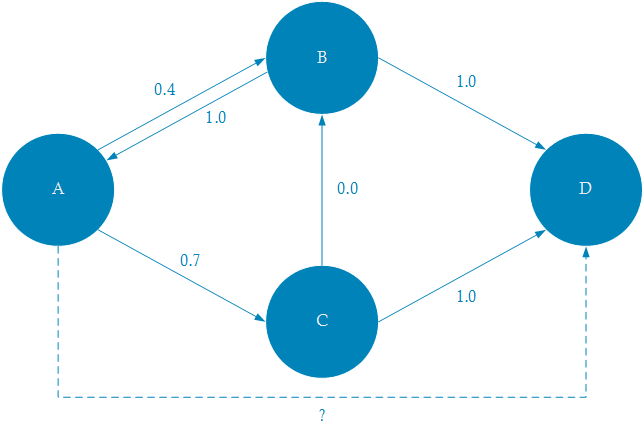
\includegraphics[width=2in]{image/webofTrust.png}
    \centering
    \caption[Trust Network]{Trust Network. Nodes are users and solid edges are trust statements. The dotted edge is one of the undefined and predictable trust statements (Adopted from \cite{Massa2004})}
    \label{figure:weboftrust}
\end{figure}

In addition to the trust network we will also have a rating matrix of size
$CxS$, where $S$ is the number of items. This rating will not differ from a
standard rating matrix, which are used in traditional collaborative filtering
systems. The value $u(c,s)$, is the rating given by user $c$ to item $s$, the
rating scale may differ from system to system.

% Architecture
The systems takes as input the trust network and the ratings matrix and
produces, as output, a matrix of predicted ratings that the users would assign
to the items. Figure~\ref{figure:trustarchictecture} shows a conceptual
overview of the trust-aware recommender system architecture.

\begin{figure}[H]
    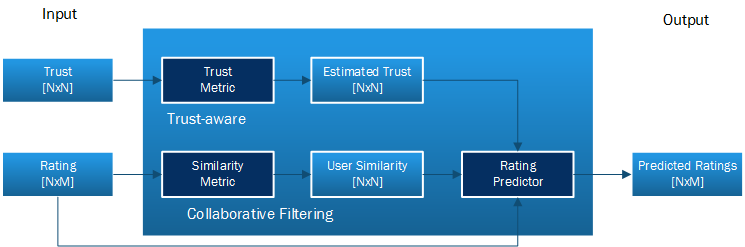
\includegraphics[width=5in]{image/trustawarearchitecture.png}
    \centering
    \caption[Trust-Aware Recommender System Architecture]{Trust-Aware
    Recommender System Architecture (Adopted from~\cite{Massa2004})}
    \label{figure:trustarchictecture}
\end{figure}

The \emph{Trust Metric} module takes the trust network as input, and exploits
trust propagation in order to predict, for every user, how much she could trust
other users. Trust metrics can either be local and global. Global trust metrics
produces an estimated trust matrix with all the rows equal, meaning that the
estimated trust in a certain user (column) is the same for every user (row). A
simple local trust metric could e.g. for each user assign to every other user a
predicted trust based on her minimum distance from the source user.

Massa et al. \cite{Massa2007} experimented with both local and global trust
metrics. The PageRank algorithm was used as a global trust metric. PageRank
tries to infer the authority of every single user by examining the structure of
the network. The algorithm follows a simple idea: if a link from user $A$ to
user $B$ represent a positive vote casted by $A$ to $B$, then the global rank
of a page depends on the number (and quality) of the incoming links. The trust
values assigned by users to users are used to predict the trustworthiness of
unknown users. Their findings, did not surprisingly, indicate that Global Trust
Metrics are not suited for the task of finding good neighbors, especially for
providing personalized recommendations, but is more suited for applications such
as \emph{Ebay.com} or similar to detect untrustworthy users. For their local trust metric
they used \emph{MoleTrust}, which is a depth-first graph walking algorithm with a tunable
trust horizon which allowed them to experiment with different propagation
distances. They found trusted users to be good predictors, especially for cold-start
users and they achieved a 63\% boots in prediction accuracy over traditional collaborative filtering
methods.

The \emph{Similarity Metric} module computes the user similarities, this is one
of the standard steps of any traditional collaborative filtering technique.

The \emph{Rating Predictor} can use the neighbors from the user similarity
matrix, the estimated trust matrix or a combination of both in order to
calculate the predicted ratings.

% Using a Trust Network to Improve Top-N Recommendation
Jamali et al. \cite{Jamali2009} propose two different methods for getting
around the cold-start user problem using a trust network. Their first approach
called \emph{Random Walk} only utilize the trust network to provide
recommendations. Starting from the active user $u$, one perform a random walk on
the trust network. Each random walk stops at a certain user. Then the items
rated highly by that user will be considered as recommended items, ordered
according to the ratings expressed by that user. Several random walks are
performed to gather more information and compute a more confident result. The
estimated rating of each item is the average of ratings for that item over all
raters considered. At the end, we output items with the highest estimated
rating as top-N recommended items. Their second approach called \emph{Combined
Approach} uses both user-user similarities and the trust network to provide
recommendations. In this approach we compute the top $K$ trusted users in the
network and rank the items rated by these trusted users to compute top-N
recommended items. The top $K$ trusted users can either be found by
\emph{Breadth First Search} or \emph{Random Walk in the social network}. We use
the collaborative filtering approach to compute another set of top-N
recommended items. Finally, we merge these two lists to produce a combined list
of top-N recommended items. Items returned by CF is denoted as $CF_{u}$, while
the items returned by Trust-based approach are denoted $TR_{u}$.

\begin{equation}
 \hat{u}(c,s) =
  \begin{cases}
   \frac{u_{tr_{c,i}}+u_{cf_{c,i}}}{2}     & i \in TR_{u};i \in CF_{u}         \\
   \hat{u_{tr_{c,i}}}                      & i \in TR_{u};i \not \in CF_{u}    \\
   \hat{u_{cf_{c,i}}}                      & i \in CF_{u};i \not \in TR_{u}     \end{cases}
\end{equation}

The top-N items with the highest value of $\hat{u}(c,s)$ will be returned as
the top-N recommended items. The authors also experimented with weighted
averaging in the case where the item appear in both $TR_{u}$ and $CF_{u}$.
Their approaches showed great improvements in recall for cold-start users,
improving the performance by 50\% over standard CF methods. The main
improvements however, are the coverage of the trust-based approaches, while
still maintaining the same or even slightly better precision than the standard
CF methods.

Papagelis et al. \cite{Papagelis2005} proposed to alleviate sparsity using
trust inferred from user-user similarity. This approach does therefore not
require users to explicitly express their trust in other
approaches described above, the trust information is inferred from the
underlying social network of the rating matrix. Their approach is based on the
assumption that the more similar two users are, the greater their established
trust would be considered.

\begin{figure}[H]
    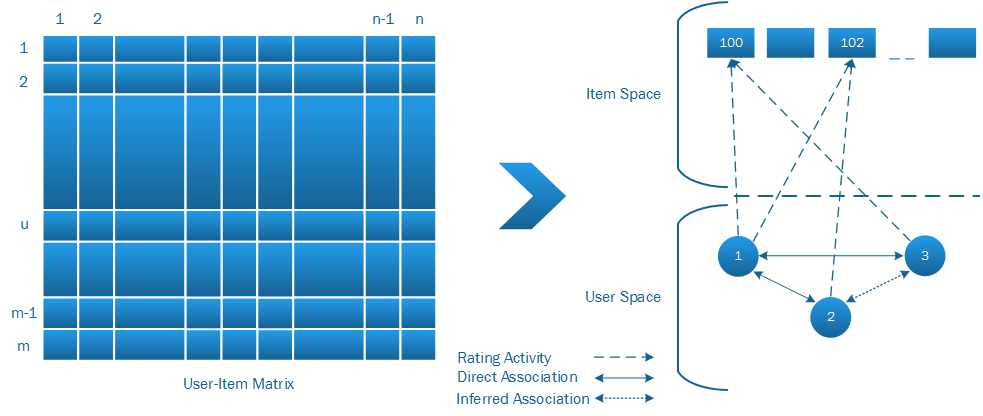
\includegraphics[width=5in]{image/trustnetwork.png}
    \centering
    \caption[Underlying Social Networks in Recommender Systems]{Underlying Social Networks in Recommender Systems}
    \label{figure:cfsocialnetwork}
\end{figure}

Due to the number of ratings that exist in recommendation systems, underlying
social networks are very sparse. There are cases in which insufficient or loss
of information is detrimental for the recommendation algorithms. Consider
Figure~\ref{figure:cfsocialnetwork}, classic CF will associate only the users
which have co-rated an item (User $1$ and $2$ and user $1$ and $3$). To deal
with the problem of a sparse social network, it is possible to infer trust
between a source user $S$ and a target user $T$ through an intermediate user
$N$ (User $2$ and $3$ are connected through the intermediary user $1$), as
shown by the \emph{Inferred Association} arrow. According to this process,
trust is propagated in the network and associations between users are built,
even if they have no co-rated item. Trust paths can be of variable length,
depending on the number of associations that one needs to traverse in order to
reach the target user.

% Trust-paths
For example, if the trust $t_{(1,2)} = 0.7$ based on 5 co-rated items
and $t_{(1,3)} = 0.35$ based on 2 co-rated items, then the trust
between user $2$ and $3$ through $1$ is, $\frac{0.7*5}{5+2} + \frac{0.35*2}{7} = 0.6$.

In order to express the subjective notion of trust, the authors set up a
confidence model that is assigned to each direct association of the network
that expresses the reliability of the association. Confidence is related to the
number of co-rated items between two users. The confidence scores are all
expressed in relation to the most confident association for each user.

\begin{equation}
c_{(s,t)} = \frac{n(I_{s} \cap I_{t})}{n(I_{s} \cap I_{u_{MAX_CONF}})}
\end{equation}

Using the above example, assuming that the maximum number of co-rated items
user $1$ has with any user is 7, $c_{(1,2)} = \frac{5}{7}$.

% Results/Findings
The authors achieved improved accuracy for all sparsity levels. With a sparsity
level of $99.9\%$ the 2-HOP CF (friend of friends) increased the MAE
performance by $17\%$ over standard CF methods.

Victor et al. \cite{Victor2008} points out that cold-start users not only have
expressed few ratings, but also typically have expressed trust in few users. In
order for trust-aware recommenders to help cold-start users they need to have
expressed trust in at least one user. But choosing who to connect to is often a
difficult task. To help cold-start users find trusted users, Victor et al.
propose using key figures or mavens (users who write many reviews), frequent
raters (users who evaluate many items) and connectors (users with
many trust connections). By connecting to these key figures, cold-start users
shown a significant increase in coverage while still maintaining good accuracy.
They also show that connecting to key figures are more beneficial to a
cold-start user than connecting to a random user.

\subsection{Filterbots}

% Na¨ıve Filterbots for Robust Cold-Start Recommendations

Park et al. \cite{Park2006} propose using filterbots to improve the cold-start
performance of collaborative filtering methods. Their filterbots are a varition
of RipperBots, described in detail in \cite{Good1999}. A filterbot is an
automated agent that rates all or most items using information filtering (IF)
techniques. The filterbots injects psuedo users or bots into the system. These
bots rate items algorithmically according to item features and user profiles.
For their movie recommendation systems the authors used 7 global bots which
e.g. rated movies based on average item rating, a critic bot that generates ratings
based on the average critic (pre-selected users) ratings, an award bot that
generates rating based on the awards a movie has won, and so on. These ratings
generated by these bots are injected into the user-item matrix along with
actual user-item ratings. Standard CF algorithms are then applied to generate
recommendations.

Their approach clearly demonstrated better robustness to all three cold-start situations than standard item-based
and user-based collaborative filtering. The improvements were most evident on
the datasets with a high degree of sparsity.

\subsection{Wisdom of the better few / Seed users}

% Wisdom of the Better Few: Cold Start Recommendation via Representative based Rating Elicitation

Liu et al. \cite{Liu2011} propose an approach in which they elect a few
representative users and items. The representative set should represent a set
of active users or items who well represent the entire population but with
little taste overlap. In their approach they wish to find a rank-k
factorization of the form $Y \approx XR$ or $Y \approx CX$ where $X$ is a
loading matrix consisting of free parameters and $R$ and $C$ which is the
component matrix consisting of actual rows or columns from $Y$. The
representative users and items are found using dimensionality reduction
techniques by reducing the column space of the rating matrix from $m$ to $k$.
And then applying basis selection based on the maximum-volume principle to
select the $k$ most representative users or items. In order to be able to
recommend new items to the users it must first be rated by the $k$
representative users, likewise for new users to be rated they need to rate the
$k$ most representative items. Their method therefore allows new users
and items to be \emph{folded in}.

\subsection{Intelligent Selection / Interview Process}\mbox{}\\

\begin{chapquote}[30pt]{Vanessa Redgrave}
  "Ask the right questions if you're going to find the right answers"
\end{chapquote}

% Getting to Know You: Learning New User Preferences in Recommender Systems

As pointed out by Rashid et al. \cite{Rashid2002}, the most direct way of
acquiring information for use in personalized recommendations from a new users
is to present item for the user to rate. However, they argue that the system
must be careful to present useful items to garner information. A fashion
recommender should probably not ask whether a new user likes any \emph{essential}
items as most users already have these items in their wardrobe. Therefore, knowing
that a new user likes an \emph{essential} item tells you very little about
the user. The choice of what questions to ask a new user, then, is critical.
The authors performed a study of different item selection strategies that collaborative
filtering recommender systems can use to learn about new users. They presented the users
with a questionnaire with items asking them to rate/select the ones they like.
Their strategies can be divided into five classes, which they evaluated based
on user effort and accuracy:

\begin{itemize}
\item Random: strategies: strategies that avoid bias in the presentation
	  of bias
\item Popularity: select among the top N items where the probability
	  that an item is selected is proportionate to the items popularity.
\item Pure entropy: present the items with the highest entropy that the
	  user has not seen
\item Balanced strategies: a balanced approach combining both popularity
	  data and entropy.
\item Personalized: as soon as some information is known about a user,
	  present items specifically tailored to that user using e.g. item-item
	  similarity
\end{itemize}

The authors found Popularity and balanced strategies to perform the best. Their
recommendation for an e-commerce recommender is to start recommending the most
popular items, rather than the highest rated ones, and then use item-item
strategies to personalize the recommendations as quickly as possible. The same
study was later extended by Rashid et al. \cite{Rashid2008} where they more
closely examined information theoretic strategies for item selection. In the
article they introduced three new strategies, which again was evaluated based
on user effort and accuracy:

\begin{itemize}
\item Entropy0: entropy Considering Missing Values
\item HELF: harmonic mean of Entropy and Logarithm of Frequency
\item IGCN: information Gain through Clustered Neighbors
\end{itemize}

The authors point out that popularity based approaches are likely to worsen the
\emph{prefix-bias}, meaning that popular items garner even more evaluations.
The accuracy differences between the approaches is fairly small, IGNC performed
the best closely followed by Entropy0 and Popularity. However, the expected
utility of the profiles built using popularity is much lower than the ones built
using information theoretic approaches.\newline

% User effort vs. accuracy in rating-based elicitation
The question then, is how many items you should ask a user to rate. Cremonesi
et al. \cite{Cremonesi2012} performed a set of experiments where they looked
at the trade-off between user-effort and accuracy. More specifically, how many
ratings are enough to provide good quality recommendations to new users? The
authors concluded that between 5 and 20 ratings are optimal for the movie
domain and that that 10 ratings is generally \emph{enough}, but that this number
depends on the recommendation method and the dataset used.

\subsection{Hybrid Methods}

Another line of search for solving the cold-start problem is to utilize
features of items and users. The content features can be used to capture the
similarities between users and items, thus reducing the amount of data required
to make accurate predictions. User data that may be collected typically
includes age, gender, nationality, marital status, income, educational level
and occupation. Item data could e.g. be the price of a product, title,
description, editorial ratings and so. The idea is that people with a more
common background share a more similar taste than someone with a random
background, and therefore good recommendations can be made as long as we know
something about the new user's background.

This section will present some latent factor models presented recently proposed
that incorporate both user/item features in addition to user-item interactions.
In Matrix factorization methods, the regularization is mostly based on a
zero-mean Gaussian prior on the factors, we refer often referred to as
ZeroMean. However in the following models the dyadic response matrix $Y$ is
estimated by a latent factor model such that $Y \approx U^{T}V$, where the
latent factor matrices, $P$ and $Q$, are estimated by regression such that $P
\approx FX$ and $Q \approx MZ$. $X$ and $Z$ denote user attribute and item
feature matrices, and $F$ and $M$ are weight matrices learned by regression.
The main difference between the following methods is how they estimate these
weight matrices.

% Regression-based Latent Factor Models

Agarwal et al. \cite{Agarwal2009} propose a class of latent factors models
called regression-based latent factor model (RLFM) that incorporates both
user/item features and past interaction data into a single model. Their
approach utilizes features of items and users as the prior distribution for
latent profiles in matrix factorization. Regularizing latent factors through
regression has important consequences when modeling sparse dyadic data. For
users/items with little data, one obtain reliable factor estimates by using the
regression estimates as a fallback. This allows the model to effectively deal
with both cold start and warm start situations. Their method assumes a Gaussian
prior, but replaces the zero mean with a feature-based regression, thus it
simultaneously regularizes both user and item factors through known features.
Users and items are anchored around a global feature-based one where profiles
are constructed by estimating deviations from the global ones in a smooth
fashion. The deviation depends on the amount of information available, e.g.
items/users with sparse data are aggressively "shrunk" to the global one. New
items and users start out with profiles based on their known features that gets
refined smoothly with the availability of more data. The model also supports
dynamic updates, which gives more weight to recent data. Their proposal is a
batched online learning scheme which updates the model on fixed time intervals
or after a predetermined amount of new observations have been made.

Their model outperformed all other models on both the MovieLens and EachMovie
datasets, and their dynamic model in particular significantly outperformed all
other models.

% fLDA: Matrix Factorization through Latent Dirichlet Allocation

Agarwal et. al \cite{Agarwal2010} propose a Matrix factorization method to
predict ratings in recommender system applications where a "bag-of-words"
representation of item meta-data is natural. Their method regularizes both user
and item factor simultaneously through user features and the bag of words
associated with each item. The key idea of their method is to let user factors
take values in an Euclidean space of existing factorization models, but assign
item factors through a richer prior based on Latent Dirichlet Allocation (LDA).
The main idea behind LDA is to attach a discrete latent factor to each word of
an item that can take $K$ different values ($K$-topics) and produce item topics
by averaging the per-word topics in the item. An article where 80$\%$ of the
words are assigned to politics and the rest to education would be though of as
a political article related to the issue of education. This allows us to model
the affinity between user $i$ and item $j$ as $s'{j}\hat{z_{j}}$, where
$\hat{z_{j}}$ is the multinomial probability vector representing the soft
cluster membership score of of item $j$ to the $K$ different latent topics.

% Matchbox: Large Scale Bayesian Recommendations
%   Online algorithm

Stern et al. \cite{Stern2009} presents a probabilistic model called Matchbox.
The system makes use of content information in the form of user and item
meta-data in combination with collaborative filtering information from previous
user behaviour in order to predict the value of an item for a user. Much like
\cite{Agarwal2009} the factors are regularized by incorporating more
flexibility in the Gaussian priors through regression on user and item factors.
Their model is dynamic, meaning that it allows an item's popularity, a user's
taste or user's personal rating scale to drift over time, as well as having the
option to be trained incrementally using Assumed Density Filtering (ADF). This
means that the value of weight matrices $F$ and $M$ will drift over time, this
is accomplished by the addition of Gaussian noise each time step. Inference is
accomplished a combination of message passing and expectation propagation.

The authors show that they can achieve state-of-the-art performance when
training the model in an on-line manner, which is especially beneficial for
dynamic domains where it is important to always have an up to date model.
Matchbox was able to train the model for the Netflix Dataset in about 2 hours
using 8 cores, meaning that it is able to add up to 14000 ratings per second.
These methods also provide quick recommendations, which is important in an
online applications, the system was able to generate 2,500,000 recommendations
in 0.25 seconds using Approximate KD Trees.

% Learning Attribute-to-Feature Mappings for Cold-Start Recommendations
%   Model for positive implicit feedback!
%   Demonstrates usefulness for new-item recommendations
%   See A. Item Recommendation from Implicit Feedback in the article for implicit feedback recommendations
%   k-NN worked best with MORE features than the linear mapping functions
%   Code can be found at: ismll.de/mymedialite

Gantner et al. \cite{Gantner2010} propose a method on how to map additional
information such as user and item features to the latent features of a matrix
(or higher dimensional) factorization model. At the core of their approach is a
standard factorization model, optimized to the recommendation task. The
extensions include a mapping function that compute adequate latent
representations for new entities from their attribute representations. This
mapping function could allow new items and users latent features to be found
only based on content-information and further on be used as if they were
normally trained latent features. The training of the factorization model with
a mapping extension consists of the following steps:

\begin{enumerate}
\item Training the factorization model using the data $S$, and then
\item Learning the mapping functions from the latent features of the entities
\end{enumerate}

The authors use BPR-MF, a matrix factorization model based on the Bayesian
Personalized Ranking (BPR) framework as their factorization model. The authors
experimented with two different ways of mapping item/user attributes to the
factor space (Only attribute-to-feature mapping for items are presented in the
article):

\begin{enumerate}
\item k-NN Mapping: Weighted k-NN regression for each factor. Determine the
k-nearest neighbors as the most similar items according to the cosine
similarity of the attribute vectors.
\item Linear Mapping: Each item factor is expressed by a weighted sum of the
item attributes. Suitable parameters for the mapping function is learned by
optimizing the model for the squared error on latent features.
\end{enumerate}

The authors found that linear mapping worked the best, and that their method
yields accuracy comparable to state-of-the-art methods.

\subsection{A Discussion on the Cold-start Solutions}
\label{sec:cold-start-discussion}

The following discussion will be based on the following points: the user-effort
required before the system can start providing high quality recommendations, the
cold-start performance of the system, how well the method fits our application
and whether or not it is a good match for our specific domain.

\subsubsection{Trust-aware recommenders}

%How can this be implemented in our system?
Requiring users to explicitly express trust, is not something users necessarily
will frown upon. Services like Instagram, Facebook and many others offers a
\emph{follow} function to their users, filling their news feeds with content from
the users which they have chosen to follow. For SoBazaar we imagine that you
e.g. could chose to follow people either because they have a good taste in
clothes or that you simply are friends, and you want to keep up with what your
friends are buying. We believe that the \emph{follow user} functionality, is
a \emph{frictionless} way of collecting high quality user information.

As previously mentioned finding trusted users can be hard. Meaning that the
application itself must be adapted to make it easy to find friends (e.g. from facebook)
which they can choose connect to. Other ways of finding users to connect to might
include \emph{most followed} users or something similarly.

As previously mentioned Massa et. al. \cite{Massa2007} found trusted users
to be good predictors. Looking directly at trusted users improved the
predictive accuracy by 62\% over traditional collaborative filtering methods
for cold-start recommendations. E.g. by using the methods described by
Jamali et. al. \cite{Jamali2009} these methods could be combined with a traditional collaborative
filtering based system to improve recommendation quality. Massa et al. \cite{Massa2004} also argue that it is more
useful for a recommender system to ask for one trust statement than asking for
one rating for new users, making it a good potential solution to the cold-start
problem given that new users of the application easily can find friends
to connect to when first using the application.

We believe trust-aware recommenders to be a good fit for the application
due to its \emph{social nature}. We believe that trust aware recommender systems
is something that should be considered at a later point when more social functionality
is in place, to further enhance the recommendation quality

\subsubsection{Interview Process}

%How can this be implemented?
Our rational behind including these articles is that we envision a simple "hot
or not" tinder like interface to be presented when new users log into the system.
You can then ask the user to "rate" e.g. 10 items by quickly \emph{swiping} them
left or right. However, requiring the user to rate rate a certain amount of items
can also be \emph{dangerous}. However, \cite{SuitUp} found that many users
enjoyed this feature.We also imagine that the tinder interface
could be available as a feature in the application for users users who just want a
fun way of browsing clothes on their mobile phone. If done right this can be
a great feature for collecting large amounts of both positive and negative feedback
from the users.

An important question to answer is how this interface will select items to
present to the user. One could either choose the simple approach of
recommending the most popular items to the user, but as previously mentioned
this is likely to worsen the prefix bias. Rashid et al. \cite{Rashid2008} got
the best results using information theoretic approaches and argues that simpler
methods such as most popular is likely to worsen the prefix bias. The authors
found Information Gain through Clustered Neighbours (IGCN) to have the best
performance overall, which they gave a maximum score for its accuracy. We choose
to ignore their user effort dimension as rating movies and clothes are two
completely different things. In order to rate a movie you must have watched
it, when it comes to clothes a quick glimpses of the item is enough.
A third strategy could be to present the newest or \emph{freshest} items
making it a fun way for users to explore the newest additions.

%Scalability & Final Verdict
We really like this approach as it is simple and elegant. Having this
functionality would make the number of user feedback available sky-rocket in addition
to providing high quality explicit feedback that is both positive and negative.
By incorporating some smart way of selecting the items which are presented
one could find ways to garner ratings for large portions of the item collection
or collecting preference data quickly about new items. However, we believe
that having negative feedback is one of the strongest arguments for applying
this method. The negative aspects of this approach is mainly limited to the fact
that it requires some active user involvement.

\subsubsection{Seed users}

In our opinion, this approach is not that suited for our domain, as it fairly
dynamic and we are working with a large and dynamic item collection. For an item to be
recommendable it must be rated by all representative users, which is highly
unlikely given the size of the item collection itself. E.g. if we have e.g. 20, 40 or 100
representative users and a spring collection is launched containing 6000 items,
for all these items to be recommendable these 15 representative users must rate
all these items. However, this method does shows some promise as a selection criteria
for items to ask the user to rate for a interview process.

\subsubsection{Filterbots}

Filterbots is a simple, but elegant solution to the cold-start problem first
presented in 1998 by Sarwar et al.~\cite{Sarwar1998}. This method
requires no user-effort other than requiring the user to rate at least one
item before recommendations can be made.
Park et al.~\cite{Park2006} clearly demonstrated the robustness of their Naive
Filterbot compared to item-based and user-based approaches in all three
cold-start scenarios. The results in \cite{Agarwal2009, Agarwal2010} also show
that the Naive Filterbots are very close to the state-of-the-art
latent factor models in terms of performance for all sparsity levels.

Filterbots could easily be implemented in any system as it only requires
the data to be run through an additional preprocessing step before it
is used to train the model. It is worth that filterbots were developed
for neighborhood models, and you can not expect getting the same kind
of performance improvements using latent factor models.

To incorporate filterbots in our system we would first have to define what filterbots
we wound want to use and what we want to achieve be using them. E.g. by using multiple
brand bots that gives each item of a certain brand a max score would make it possible to give brand specific
recommendations as soon as a user have expressed preferences for an item, thus connecting
him to a filterbot with high ratings for all items of the given brand. Similarly
a \emph{PopularityBot} would \emph{recommend} the most popular items to users which
they are connected to. These bots can therefore be made to capture the general underlying
trends of the users or give recommendations based on content-features of the items.
Given that we use the bots mentioned above, as soon as a new user rates a single item
rated by both bots he would theoretically be recommended the most popular items of
the brand which she expressed her preference for, making it a potentially good fit for fashion
recommendations.

\subsubsection{Hybrid recommenders}

Latent factor models are currently the main paradigm within the recommender
system field and are currently considered the state-of-the-art recommendation
methods. The all the hybrid methods achieved state-of-the-art performance as well as
having good fallback methods based on user and item features to solve the
cold-start problem. In addition to incorporating item-features and/or user-features
these models also incorporate some notion of recency, reducing the importance of
items over time. Another advantage of these models are that they support
online training of the models, which further could improve the cold-start
performance by \emph{instantly} incorporating new preferences.

In order to implement these recommender we would first need access to
high quality item and user-features. The item-attributes could be extracted
from the product database, which demographic information could e.g. be
extracted from Facebook data. Another concern of ours is that our dataset is
currently to small for latent factor methods, since most of these methods
rely on binary data (e.g. purchases only) to provide recommendations.

\subsubsection{Summary}

It is hard to compare the performance of the different methods as the authors have
experimented with different datasets and evaluation measures making it hard to do
a quantitative comparison. We therefore opted to do qualitative assessment of the methods
in question. It is worth nothing that qualitative methods are less about attempting to prove
something than about to understand something. Our ordinal rating scale spans from \ding{55} meaning
\emph{bad}, \checkmark means \emph{good} \ding{55} and finally \checkmark\checkmark means \emph{best}


\begin{table}[H]
    \centering
    \begin{tabular}{*{4}l}
    \toprule
    Method					& Cold-start performance  & User-effort \\ 			\midrule
    Trust-aware RS 			& \checkmark			  &	\ding{55}				\\
    Filterbots 				& \checkmark			  &	\checkmark\checkmark	\\
    Seed users 				& \checkmark			  &	\ding{55}				\\
    Intelligent selection 	& \checkmark			  &	\checkmark				\\
    Hybrid Methods 			& \checkmark \checkmark	  &	\checkmark\checkmark	\\
    \bottomrule
    \end{tabular}
    \caption[Evaluation of cold-start methods]{Evaluation of cold-start methods}
    \label{table:evaluationcoldstart}
\end{table}

Trust-aware recommender systems get a \ding{55} in user effort as it is hard to find users to connect to,
this problem could however be mitigated by implementing a system like the one described by Victor et al. \cite{Victor2008}
to recommend users to connect to. Seed users also get a \ding{55} in user-effort, mainly due to its solution to the new item
problem where all representative users must rate an item for it to be recommendable. Filterbots and the Hybrid methods both
get two checkmarks for requiring no extra user involvement. Intelligent selection could pretty seamlessly be integrated into
the solution using e.g. a simple \emph{hot or not} interface, requiring minimal user effort. We would also like to argue that having the
option to incrementally update the model is an important feature which could further improve cold start performance, as it instantly can
incorporate the ratings given by new users and to new items. The hybrid methods therefore gets to checks for their cold-start performance.

From our discussion we believe filterbots, interview process and hybrid methods such as e.g. RBLF and MatchBox could provide good solutions.
However, we are currently limited to experiment with filterbots as we do not have access to user and item features or any way
of testing out an interview process.

% !TEX root = ../../report.tex

\clearpage

\section{Implicit Feedback to Implicit Ratings}
\label{sec:implicit}

In this section, in accordance to our research goals (\textbf{Goal G6 and G7}),
we will explore several \textit{existing} methods for solving the following
formalized problem:

\vspace{5 mm}

\noindent \textit{Input:} A dataset with \textbf{implicit feedback} containing event logs
with the following information available: event type, product id, user id and
timestamp of the event.

\vspace{3 mm}

\noindent \textit{Output:} For every user $u$, a rating between 1 and $k$ on every item that
the user has interacted with. These ratings are called \textbf{implicit
ratings}.

\vspace{5 mm}

This problem definition is further used in
Section~\ref{sec:implementation-implicit} where multiple ways of quantification
of the SoBazaar dataset are presented based on ideas found in this section.
First however, before delving into specific methods, a deeper understanding on
the relationship between implicit and explicit feedback is needed.

Explicit feedback is present in many of the largest recommender systems today
and hence, is extensively researched \cite{Adomavicius2005}. The user is
commonly asked to rate item $i$ on a Likert scale from $1$ to $k$, ranging from
strongly disagree to strongly agree with an item. Its advantages are, among
others the ability to get precise feedback from the user and capturing both
positive and negative preferences. However, although having a high popularity,
the method has multiple weaknesses. The most prominent weakness is the
difficulty of collecting ratings: the method requires the user to spend time
rating items and the amount of feedback is often scarce, creating sparse data
sets. Further, explicit ratings are often subject to inconsistencies known as
natural noise~\cite{amatriain2009like} and users might also be pressed to
report different preferences due to peer pressure \cite{bell2007scalable}. The
fact that we are introducing a user overhead, makes it difficult to have a
complete view on the user preferences~\cite{Jawaheer2010}.

There are also practical reasons for not having explicit feedback in form of
ratings, dependent on how a website/application interacts and works with its
customers. One of the most popular recommender sites in the world, Netflix, ask
their users to rate items after consumation. However, this process does not
\textit{cost} anything for the user, and the possibility to rate is included in
the monthly subscription price, whilst in a webstore rating an item often
require the user to first buy it, consume it and finally rate it.

Implicit feedback on the other hand utilizes, often already collected,
analytics data and hence does not require any extra effort neither for the user
nor the frontend-developers. This creates a more frictionless experience for
the user, but can also yield better recommender results since often the event
log is less sparse than rating datasets and contains implicit knowledge which,
by only using explicit information, would never be exposed in a traditional
system.

It is important to understand that there are several fundemental differences
between implicit and explicit ratings, in everything from \textit{meaning} to
\textit{evaluation techniques}. Partly inspired by Hu et al.~\cite{Hu2008}, we
can identify the following key charecterstics and differences between them:

\vspace{3 mm}

\textbf{Explicit ratings:}
\begin{itemize}
\item Contains both positive and negative feedback. In other words, a user is
able to explicitly tell the system that he/she does not like an item, as well
as the opposite.
\item Indicates preference, often on a Likert scale (or similar), where scores
range from total dislike to high satisfaction with an item.
\item There is medium noisiness in the data, but the amount is highly dependent
on the domain in question~\cite{amatriain2009like}. With little noisiness we
achieve more precise ratings.
\item Metrics in use are commonly RMSE, MAE or other evaluation schemes where
we consider how well we match a test-set.
\item Both evaluation schemes and recommendation techniques using explicit
feedback is heavily researched and used. Many of these are easy to implement,
and multiple open-source tools and projects are at researchers and developers
disposal~\cite{mahout}~\cite{Gantner2011MyMediaLite}.
\end{itemize}

\textbf{Implicit ratings:}
\begin{itemize}
\item Usually only contain positive feedback, since we base our models on user
activity on an item representing something good. However, looking at metrics
such as bounce rates so forth, negative feedback can be produced with some
effort.
\item Indicates confidence, that is a recurring event is more likely to reflect
the user opinion, but not necessarily his/hers preference.
\item There is a high degree of noise and this is one of the main challenges
with implicit rating and its precision. Researchers and developers need to be
sure to select correct set of events and session-metrics to base implicit
ratings on.
\item As users do not provide numerical scores, a precision-recall evaluation
scheme is often preffered to more preference-based metrics.
\item Strengths include not requiring extra feedback for the user, having less
sparsity and catching actual behaviour in the application. Less influenced by
peer pressure and so forth.
\end{itemize}

Notice that several events such as purchasing an item may be considered as
explicitly giving positive feedback, but as we argue in this paper all events
in the SoBazaar dataset (including purchases) are treated as implicit feedback.
The reasoning behind this lies in the fact that purchasing, in contrast to
positivly rating, an item happens before actual consumption. Hence the user may
not like the item in question, it may be a gift for another person or a variety
of other reasons. Whilst in the scenerio of rating, the user has already
consumed it and is explicitly answering the question \textit{«To which degree
did you like it?»}.

\clearpage
\subsection{Binary implicit ratings}
\label{implicit-als-wr}

One of the most common techniques of quantifying implicit feedback to implicit
ratings is to use binary ratings - that is if a user has shown any interest in
an item we give that item a weight of 1, similarily all items the user has not
shown interest in (e.g. not clicked on) we give a rating of 0. This method was
introduced and used by Hu et al.~\cite{Hu2008} where they formalized the
notion of confidence which the $r_{ui}$ variables measure, e.g. if a user $u$
had clicked on an item $i$ 2 times it would translate to the score $r_{ui} =
2.0$. This was further converted to a $p_{ui}$ value derived by binarizing the
$r_{ui}$ values:

\begin{equation}
  p_{ui} =
  \begin{cases}
    1 & \text{if $r_{ui} > 0$} \\
    0 & \text{if $r_{ui} = 0$}
  \end{cases}
\end{equation}

As mentioned earlier in this section, and as it is also noted in the original
research, when we have implicit rather than explicit feedback there may be
multiple reasons beyond preference that decide consumation of an item. It may
be due to the items availability or price; the users knowledge of the item
caused by e.g. the user interface or one of many other factors different from
the user preferring or disliking the item. To remidate this they introduce a
variable $c_{ui}$ which measure the confidence in observing $p_{ui}$, where
their main hypothesis is that as the $r_{ui}$ grows the confidence is stronger.
Hence, a plausible choice for $c_{ui}$ would be:

\begin{equation}
c_{ui} = 1 + \alpha r_{ui}
\end{equation}

Where $\alpha$ controls the rate of increase, and is set to $40$ in their
experiments as this produced good results. They now use these two scores
($p_{ui}$ and $c_{ui}$) in parallel when finding latent factors and training
their model. In short they find both a user and item vector ($x_u$ and $y_i$,
respectively) where the preference is assumed to be their inner product: $p_{ui}
= x_{u}^{T} y_{i}$. Notice as well how this method stand out from similar
matrix factorization methods (see Section~\ref{sec:model-based-methods}) by
accounting for varying confidence levels:

\begin{equation}
  min_{x,y} \sum _{u,i} c_{ui} (p_{ui} - x_{u}^{T} y_i)^2 + \lambda (\sum _{u}
  || x_u ||^2 + \sum_{i} || y_i ||^2)
\end{equation}

Where the $\lambda (\sum _{u} || x_u ||^2 + \sum_{i} || y_i ||^2)$ term is
necessary for regularizing the model, so that is will not overfit the
training data. $\lambda$ is highly data dependent and should be set by
cross-validation.

However, notice the primary term where the difference between the binary weight
and our user/item-models are minimized and perhaps more importantly multiplied
by our confidence. As the details on this topic are quite detailed and diverges
a bit from the generation of implicit ratings, we will stop our analysis of it
here. But is shows an important aspect which we will return to in subsequent
sections, namely the confidence in repetitive events and our continuous
challenge to obtain higher confidence in our implicit ratings. For further
information on matrix factorization and latent factors refer to
Section~\ref{sec:model-based-methods} or to Hu et al.\ original
research~\cite{Hu2008}.

\subsection{Implicit ratings for binary domains}
\label{implicit-binary-domains}

In the previous sub-section we saw how $r_{ui}$, a score for user $u$ on item
$i$, was set based on e.g. number of clicks but perhaps more commonly the
duration or amount of which the user has consumed the item. This way, in a
domain such as television a user would obtain $r_{ui} = 1.0$ if the whole
programme was watched, and similarily $r_{ui} = 0.5$ if half of the show was
watched, and so forth. Now, this works well in domains where actions on an item
are continious, but in many domains such as a e-commerce store we mostly have
binary events such as clicks or purchases. One scheme, proposed by
~\cite{pkghost2014implicit} is to differentiate between different events and by
weighting these by importance or relevence we can create ratings using the
whole scale between 0.0 and 1.0.

This is just one example of how the domain and data available affects our
methods, techniques and reliability to our predicted numbers. This is common
theme when dealing with implicit ratings, and it is an important aspect that
the reader should be aware of and keep in the back of his/hers mind. Now, in a
proposed e-commerce domain where our data is based on web-access logs we may
have the following events to choose from:

\begin{table}[H]
  \centering
  \begin{tabular}{ll}
  \toprule
  Event type & Description \\ \midrule
  0 & Item purchased \\
  1 & Item placed in shopping cart \\
  2 & Item placed in wish list \\
  3 & Item browsed based on search result \\
  4 & Item browsed \\
  \bottomrule
  \end{tabular}
\end{table}

Then, our heuristic would count the frequency of each event for an item $i$ on
user $u$. However, just counting is not a bounded function -- so if one give
\textit{Item browsed} the weight of $1$ and the \textit{Item purchased} event
a weight of $100$, then a user browsing an item more than 100 times would get a
higher implicit rating than a user buying it.

Instead,~\cite{pkghost2014implicit} proposes using a global rating mapping,
that uses \textit{levels of frequency}.

\begin{table}[H]
  \centering
  \begin{tabular}{ll}
  \toprule
  Event type & Scores \\ \midrule
  0 & 100 \\
  1 & 70, 77, 80 \\
  2 & 30, 40, 45, 48, 50 \\
  3 & 20, 25, 28, 30 \\
  4 & 10, 15, 18, 20 \\
  \bottomrule
  \end{tabular}
  \caption{Scores per event type, increases as frequency of each event
           increments}
\label{implicit-table}
\end{table}

Now, a user browsing an item $i$ two times, would get a score of 40 and a if
buying it the score would be 100 (e.g.\ the event type with highest interest
level supersede all others). Equally, if a user browsed the item 100 times, it
would make no difference in score compared to browsing it 4 times. The scores
given to the various event types may vary from what kind of dataset one have,
the domain and should be evaluated using one or more of the methods mentioned
in Section~\ref{sec:evaluation}.

If we wanted ratings between 1 and $k$ one can transform the score $s$ provided
by Table~\ref{implicit-table}:

\begin{equation}
  ImplicitRating(s, k) = 100 * \frac{k-1}{100} + 1
\end{equation}

The advantage of this heuristic is that it requires no training, it is simple
to understand and works reasonably well, if weights are chosen correctly.
The latter is also its largest weakness -- as finding these weights may be
difficult. If one had explicit feedback, as well as the implicit, one could
train a model automatically choosing weights. Further, when using the scores
defined as above we only use a small percentage of the scale 0-100. This leads
to problems when a user triggers one type of event many times more than
another, as both would reach the highest score of the given event type, but
there would be no difference in scoring even though they had very different
activity. We would like a scheme where we use the whole scale of scores and
where there were no global ceiling, but rather let the scoring be normalized to
the number of events for the user in question.

Improvements to this model are presented in
Section~\ref{sec:implementation-implicit}

\subsection{Regression analysis}
\label{sec:regression-sota}

\paragraph{Introduction to linear regression}
A different method for converting events to ratings is finding a mathematical
model which fits our observed data. Using this model we can predict new ratings
by extrapolation or intrapolaton. Our observed data can be in N-dimensions, but
in the figure below we consider two dimensions of observed properties, in which
the goal is to find a regression line matching the data points with minimal
errors. An example regression line matching five data points is provided below:

\begin{figure}[H]
  \centering
  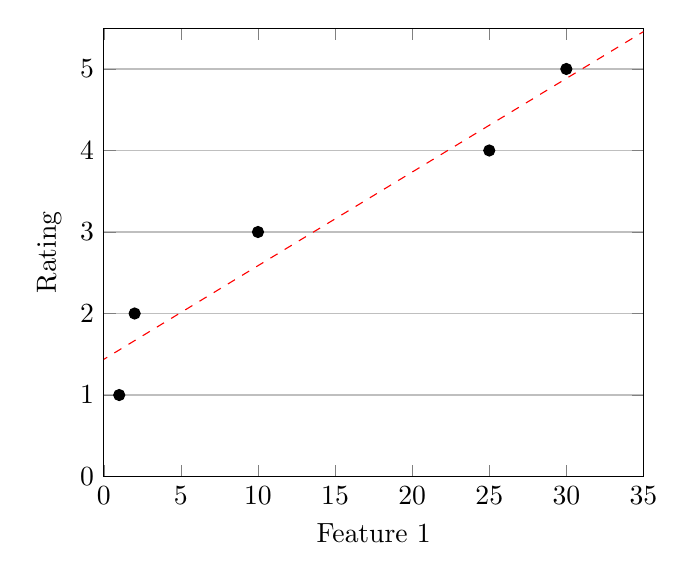
\begin{tikzpicture}
    \begin{axis}[
        xlabel=Feature 1,
        ylabel=Rating,
        ymax=5.5, ymin=0,
        xmax=35, xmin=0,
        ymajorgrids=true,
    ]
    \addplot[only marks]table[]{
      1 1
      2 2
      10 3
      25 4
      30 5
    };
    \addplot [dashed, color=red, domain=-3:35, samples=40] {0.114861*x + 1.437889};
    \end{axis}
  \end{tikzpicture}
  \caption{Regression line fitting the 5 observed datapoints}
  \label{fig-regression}
\end{figure}

In this example we consider the relationship between one feature (the
independent variable) and the rating (ground truth/dependent variable), using
five observed datapoints. We can then, given a feature-value, predict future
ratings. The process of finding the regression line is better generalized by
solving the following equation, where we are given a number of independent and
dependent values:

\begin{equation}
  \hat{y}(w,x) = w_0 + w_1 x_1 + \cdots + w_p x_p
  \label{eq-regression}
\end{equation}

where we want to find the values of the $w$-parameters, also called the unknown
parameters. This is done by using multipe known values for $x$ and $y$, the
independent and dependent variables respectivly. In Figure~\ref{fig-regression}
we have the following datapoints:

\begin{table}[H]
  \centering
  \begin{tabular}{ll}
  \toprule
  Feature-value (x) & Rating (y) \\
  \midrule
   1 & 1 \\
   2  & 2 \\
   10  & 3 \\
   25 & 4 \\
   30  & 5 \\
   \bottomrule
  \end{tabular}
\end{table}

Which, solving Equation~\ref{eq-regression}, five different equations are
used with the unknown parameters $w_0$ and $w_1$:

\begin{equation}
  \label{eqs-regression-example}
  \begin{split}
    1 = w_0 + 1 w_1 \\
    2 = w_0 + 2 w_1 \\
    3 = w_0 + 10 w_1 \\
    4 = w_0 + 25 w_1 \\
    5 = w_0 + 30 w_1
  \end{split}
\end{equation}

Using a minimization method called \textit{Least squares} we try to minimize
the residual $e = y_i - w^{T}x_{i}$, using sum of squares between the observed
values in the dataset and the values predicted by the linear approximation. In
other words we want a minimal distance between all observed datapoints the the
final regression line. Mathematically it solved the problem of the following
form:

\begin{equation}
  \label{least-squares}
  \hat{w} = \argmin_w \sum_{i} (y - w^{T}x_{i})^2
\end{equation}

Carrying out this minimization for our equations~\ref{eqs-regression-example},
we obtain an intercept value ($w_0$) of $1.4379$ and a slope ($w_1$) of
$0.1149$, which matches the regression line plotted in
Figure~\ref{fig-regression}. Predicting a new rating based on a feature value
in now very simple - as an example we assume a new independent value is
provided with the value 15 and an unknown rating, that is $x=15$ and we can
solve the equation $y = 0.1149 \cdot 15 + 1.4379$ which yields the $y$-value or
rating $3.1614$.

\paragraph{Using regression analysis on implicit feedback}
The process of using regression analysis in order to predict ratings based on
implicit feedback has already been done in a different domain, by Parra et
al.~\cite{parra2011walk}. Where they first did a quantitative user study
asking 114 active users of the music service Last.fm to rate items which was
found in their activity history. These ratings were used as dependent variables
and then using various schemes described below they, mapped these to the
independent variables. Now, a key point in their study is the fact that all
models found used explicit feedback from a user study as a \textit{ground
truth}. The necessity of such a ground truth is the largest weakness in terms
of regression analysis on implicit datasets - as it is per definition
non-existent. A possibility is to give various events scores based on
importance in the system, with e.g. a purchase having top-score and clicking on
an item a low score. This is discussed further in Section~\ref{} where an
implementation and evaluation of such a design is presented as well.

The study looked at three different features for each item, found in the
dataset:

\begin{itemize}
  \item User activity on the item
  \item Global popularity of the item
  \item How recent the user had activity on the item
\end{itemize}

For each feature all items are categorized into three buckets, so that items
are equally distributed across one feature. Thus bucket one for the feature of
global popularity contains items with low popularity and bucket three those
with the highest popularity, and so forth. The main reason for having this
sampling strategy is to create a homogenous set of items where outliers are
accounted for, and we are less prone to over or underfitting.

Four models are proposed, utilizing the features above and the ratings provided
in the user study:

\begin{equation}
  \begin{aligned}
    & r_{iu} = w_0 + w_1 if_{iu} \\
    & r_{iu} = w_0 + w_1 if_{iu} + w_2 re_{iu} \\
    & r_{iu} = w_0 + w_1 if_{iu} + w_2 re_{iu} + w_3 gp_{i} \\
    & r_{iu} = w_0 + w_1 if_{iu} + w_2 re_{iu} + w_3 if_{iu} \cdot re_{iu}
  \end{aligned}
\end{equation}

where every independent variable ($if_{iu}$, $re_{iu}$ and $gp_{i}$) is the
bucket number between 1 and 3. $if_{iu}$ indicates how many times user $u$ used
item $i$, $re_{iu}$ how recently user $u$ used item $i$ and $gp_{i}$ the global
popularity of item $i$.

Evaluating a regression model is done by confirming the \textit{goodness of
fit}, and the most common metric is to calculate the $R^2$ which based on
residual values in Equation~\ref{least-squares} yields a number between 0 and
1, indicating a bad or good fit, respectivly. By accounting for recentness in
their regression model (model 2\-4) they achieved an improvement in the $R^2$
value by \textit{10\%}.

Summarizing, the following requirements are needed in order to perform
regression analysis on implicit feedback:

\begin{itemize}
  \item A ground-truth score.
  \item A set of numeric features.
  \item Each feature have to be transitive, that is a linear relationship in
  the values have to exist.
\end{itemize}

The fact that the features have to be transitive implies that one can not use
e.g. \textit{item category} as training feature, unless the brands (or rather
the brand ids) themselves are sorted by price or equality, then renumbered.

\paragraph{Multivariate ordinal regression}
In~\cite{parra2011implicit} Parra et al. extend the model presented
in~\cite{parra2011walk} by considering that the dependent variable (rating) is
on an ordinal scale, that ranges from 1 to 5. A ordinal variable implies that
the numeric value has no significance beyond its ability to establish a ranking
over a set of data points. When solving regression problems on an ordinal scale
a logistic function is commonly used. Further since there exists more than two
outcomes (1 to 5) they use a multinomial regression type.

In \textit{multinomial logistic regression} problems such as this, the link
function (logistic function, also called \textit{logit}) is trained based on
features found in the data. In the refered study they examine the music domain
and hence they include listen count, recentness and the global popularity as
features to the link function.

When trained they have a probability function for all discrete outcomes and can
thus based on model input obtain a value between 0 and 1, indicating the
probability of the enquired outcome. The final rating is then calculated as:

\begin{equation}
  E[r_{ui}] = \sum_{k=1}^{5} k \cdot P(r_{ui} = k)
\end{equation}

where $u$ and $i$ is the user and item in question, respectively. $k$ is the
ordinal variable between 1 and 5, and $P(r_{ui})$ yields the probability of $k$
being the rating for item $i$ on user $u$.

This model yields an improvement in performance both measured in MAP and
nDCG-scores (see Section~\ref{sec:evaluation}), compared to their previous model. However,
when they discuss the accuracy of their evaluation metrics a conclusion is made
which is similar to what is laid out in this thesis as well:

\begin{quotation}
  [\dots], we do agree that there is no appropriate evaluation approaches for
  implicit feedback.
\end{quotation}

Their proposed method for evaluation is to compare the generated implicit
ratings to ones given in a parallel explicit scenario. However, in many
situations where the two techniques are not combined, we use implicit ratings
due to the lack of explicit ones. Consequently, without any ground truth (that
is, explicit ratings) both \textit{training a regression model} and
\textit{evaluating} the generated implicit ratings becomes difficult. If one
wants to reliably use these two methods a user study should be conducted, which
was not performed in the case of SoBazaar due to time and user constraints.

\subsection{Relative preferences using buying frequency}
A hybrid approach using sequential pattern analysis and collaborative filtering
techniques is presented by Choi et al.~\cite{choi2012hybrid}. In their
method, coined HOPE, they calculate an implicit rating by finding the
absolute preference $AP$ from users and items. These preferences are further
used to find the relative preference which finally are normalized into an
implicit rating. Once the implicit ratings are derived they calculate
similarity scores and find K-nearest neighbours in a traditional fashion.
Finally these neighbours are used in order to calculate a CF-based predicted
preference (CFPP). This score is integrated with a Sequential Pattern
Analysis-based predicted preference (SPAPP) which is derived from matching
subsequences of common sequential patterns between users. This process is
summarized in Figure~\ref{hope-system}.

\begin{figure}[H]
  \centering
  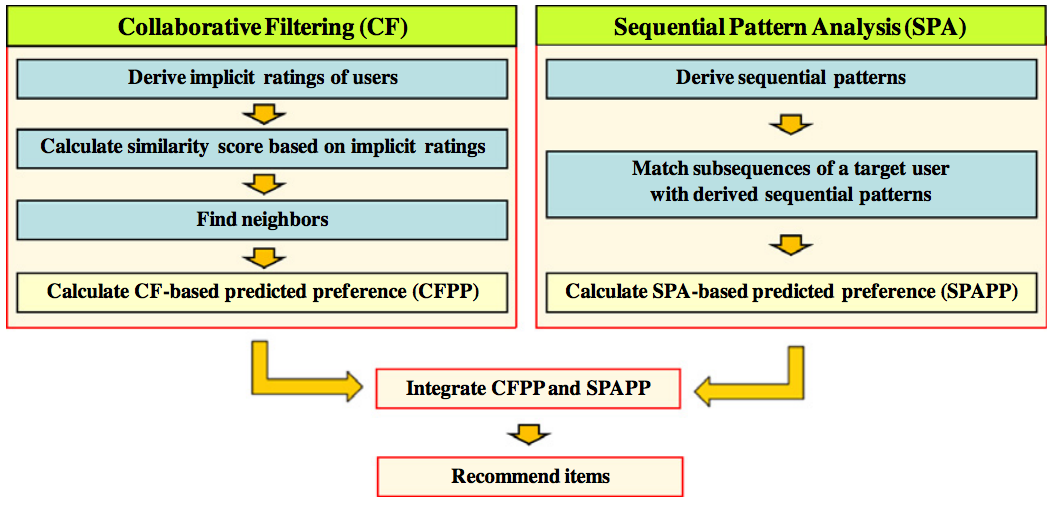
\includegraphics[scale=0.3]{image/hope-system}
  \caption{Overall framework of HOPE system, calculating implicit ratings and
  combining these with sequential pattern analysis}
  \label{hope-system}
\end{figure}

We will continue this section focusing on the convertion from transaction data
into implicit ratings, rather than going in depth into sequential pattern
analysis and calculating the CFPP and SPAPP-scores, as the interested reader
rather should consult the original research for a indepth discussion. When
calculating the $AP$ score we focus solely on the purchase data of the user
$u$, but it can easily be extended to other types of events. However, the score
does makes more sense when using it on domains having a high degree of repeated
actions - such as e-commerce stores selling convienience products with short
life spans or a music service having users listening to a song multiple times.
The absolute preference is calculated as follows:

\begin{equation}
  AP(u,i) = \ln(\frac{trans(u,i)}{\sum_{e \in E}{trans(u, e)}} + 1)
\end{equation}

where $trans(u,i)$ is the number of transactions for user $u$ on item $i$, and
E is the set of all items in our system. As an example if a user $u$ purchases an
item $i$ four times out of ten transactions the $AP(u,i) = \ln(1.4)$, but another
user $p$ who has bought the same item one time out of one transaction the
$AP(p,i) = \ln(2.0)$, and as one can see we should consider a relative preference so
that repeated actions are rewarded. Further, the absolute preference only takes
into account the frequency of purchases and because the frequency is heavily
dependent on price, item category and lifespan of an item — so in the original
research they propose the following equation in order to calcualte the relative
preference@:

\begin{equation}
  RP(u,i) = \frac{AP(u,i)}{\max_{c \in U}(AP(c,i))}
\end{equation}

where $U$ denotes every user who purchased item $i$. The reason for using a
maximization function, is to make $RP(u,i)$ range from $0.0$ to $1.0$ (i.e.\
normalization) and one can thus find a rating on a common Likert scale by
multiplying with $k$:

\begin{equation}
  ImplicitRating(u,i) = \lceil k * RP(u,i) \rceil
\end{equation}

Here we round up in order to range from 1 to 5, but one could either round down
instead and have ratings range from 0 to 4 or one could use the normalization
equation where we based on minimal and maximal values in an interval $x_{min}$
and $x_{max}$ shift all values to a new interval $a$ and $b$, keeping the
ratios between items. Using this equation we can normalize any $x$ defined in
the interval, that is $x_{min} \leq x \leq x_{max}$:

\begin{equation}
  \label{eq-normalization}
  N(x, a, b, x_{min}, x_{max}) = a + \frac{(x-x_{min})(b-a)}{x_{max}-x_{min}}
\end{equation}

In order to normalize $ImplicitRating(u,i)$ we set $x_{min} = 0$ and $x_{max} =
1$ and normalize to the new interval $a=1$ and $b=5$.

\subsection{Challenges and weaknesses}
\label{implicit-weaknesses}

At this point we have looked at multiple existing methods for creating implicit
ratings based on implicit feedback, proving both their extensibility and
numerous variations. However, there are some challenges and weaknesses that
holds true for all methods. We will take great care to explain these, but in
addition describe the multiple ways of counteracting or minimizing their
impact as well. The two largest challenges in regards to generating implicit
ratings are:

% Goal G9: Find metrics in order to evaluate the implicit ratings.

\begin{itemize}
  \item A lack of ground truth.
  \item No negative feedback.
\end{itemize}

% First challenge, the lack of ground truth.
As mentioned in Section~\ref{sec:regression-sota}, when discussing regression
analysis, without a ground truth both modeling and evaluating becomes a
inaccurate science based on assumptions. Some assumptions may very well hold
true, as proved by in~\cite{parra2011walk}, however without conducting user
studies or evaluating the implicit ratings in an online environment using
conversion metrics such as an increase in purchases, we can not reliably
evaluate our results. We can thus calculate and compare the performance of one
set of implicit ratings compared to another set of implicit ratings, but only
based on how well they \textit{match our assumptions} and selected features,
not their real world performance. This in many answers, but also make it
irrealizable given our data, to fulfill our research goal concerning finding
good metrics for evaluating the implicit ratings (\textbf{Goal G9}) as we
neither have a ground truth, nor a set of explicit ratings from the
application.

% Second challenge, no negative feedback.
The second challenge is a result of almost all research on implicit feedback
focusing on how implicit behaviors can be used as positive evidence in a
recommender system. Without any negative feedback direct comparisons to
explicit ratings become troublesome, as an implicit rating of 2 does not mean
\textit{dissatisfaction}, but instead only \textit{less} satisfaction than 3.
By adding negative events to implicit rating generation such as \textit{bounce
rates} or \textit{deleting/hiding} elements from a news feed, may improve both
the accuracy of the ratings, but also make them more robust when comparing and
combined with explicit ratings. Still, dependent on the domain, these negative
implicit feedbacks are often fewer in number and demand a larger effort to
extract.

% Other challenges; making too many generalizations on user behaviours.
There are many other smaller challenges when generating implicit ratings, one
of them concerning making too many generalization rules for user behavior. In
particular, users behave differently and have varying approaches to information
seeking, thus it becomes difficult to generate and dangerous to apply
all-purpose rules for describing their behavior. This way, individual
differences can greatly impact the effectiveness of analyzing user behaviors,
which is at the core of our assumptions.

% Weaknesses propagate, and recommender+evaluation is based on impl. feedb.
When we create implicit ratings, these become the recommender system equivalent
of a ground truth. This data is further used, as we have seen in
Section~\ref{subsec:cf} as input to our recommender algorithm makes which makes
creates a model and later gives predictions on how well new data fits this
model. In the end we use the output from this model (the predictions) for
evaluation, determining the quality of how well the predictions were. However,
notice that if all input to creting the \textit{recommender model} were
unaccurate or wrong, then this would affect all later stages in the
\textit{recommender pipeline}. This is generally not a concern in explicit
ratings, after all the ground truth is the \textit{truth}, but when considering
implicit ratings it can instead be called the \textit{ground assumptions} and
if wrong, all later stages become unsound as well. Furthermore, as briefly
touched upon earlier, without much negative feedback our later stages in the
pipeline need to take height for this, not penalizing a low ranking as much as
in traditional settings -- as having some feedback is better than none. In
essence, we need to ensure that two factors are emperically chosen: first, all
assumptions should be grounded in statistical evidence and second, recommender
algorithms and evaluation schemes should take height for weak evidence of
negative feedback.

% We need in-depth understanding of the domain.
A consequence of using implicit ratings is therefore to statistically select
features that yields a good classification of user behaviours. In addition,
we need to consider the sparsity of the dataset and dependent on the domain
filter out implicit feedback based on criterias such as time sensitivity or
others. This is seen in the fashion domain, where we after some time want to
expire the implicitly provided feedback, as a users taste and preferences
constantly changes, as well as the current fashion trends. In other words an
\textit{in depth understanding of the domain} is required, and should be
ensured by answer a set of research goals before designing and implementing a
implicit rating system (See research goals \textbf{G1, G2 and G3}).

% !TEX root = ../../report.tex
\section{Evaluating recommender systems}
\label{sec:evaluation}

% Refering to research goals and defending why we need this section.
Our research \textbf{goals G5 and G8} requires us to identify existing metrics
for evaluating recommender systems in a sparse dataset with implicit feedback.
Set forth by our problem statement we need to propose one recommender system,
selected from a range of candidate approaches and techniques. We recall our
system overview in Figure~\ref{fig:system-overview} where in the last step of
the pipeline we \textit{evaluate} our recommendations. There are a range of
different metrics for ranking the performance of recommender systems, and they
are all highly dependent on which properties the system designer prioritizes as
important for both the domain and application.

% Explaining basic difference between offline/online eval.
There are mainly two settings for doing evaluation experiments. First is doing
them \textit{offline} where the system is evaluated without user interactions.
Second is, not surprisingly, \textit{online} evaluation, where real users
interact with the system. In this thesis we did not have the possibility to
perform any online evaluations, and hence a larger focus will be given to the
offline setting.

% Refer to Appendix for more evaluation metrics, only focusing on suitable here.
There exists too many evaluation metrics to describe them all in this thesis,
consequently in this section we focus on the ones suited for our needs – that
is, extremely sparse implicit ratings in the fashion domain. A comprehensive
study of non-suitable solutions were performed as well, and can be found in
Appendix~\ref{appendix:evaluation-metrics}.

% TODO: We don't refer to these steps, so perhaps just skip them?
% Shani et al.\ \cite{Shani2011} lists the following guidelines for general
% experimental studies:
%
% \begin{itemize}
% 	\item Hypothesis: before running an experiment one must form an hypothesis. For
% 		example, an hypothesis can be that algorithm $A$ better predicts user ratings
% 		than algorithm $B$. In that case the experiment should test the prediction
% 		accuracy, and not look at other factors.
%
% 	\item Controlling variables: when comparing a few candidate algorithms on a
% 		certain hypothesis, it is important that all variables that are not tested
% 		are fixed.
%
% 	\item Generalization power: when drawing conclusions from experiments, we may
% 		wish that our conclusions generalize beyond the immediate context of the
% 		experiments. When choosing an algorithm for a real application, we may want
% 		our conclusion to hold on the deployed system, and generalize beyond the
% 		experimental data set. To increase the probability of generalization of the
% 		recommender results one must typically experiment with several data sets or
% 		applications.
% \end{itemize}

\subsection{Offline evaluation}

Offline experiments are performed using pre-collected datasets and a protocol
that models the user behavior to estimate recommender performance through
different evaluation measures. The following figure shows a \emph{traditional}
offline evaluation pipeline:

\begin{figure}[H]
		\centering
	  	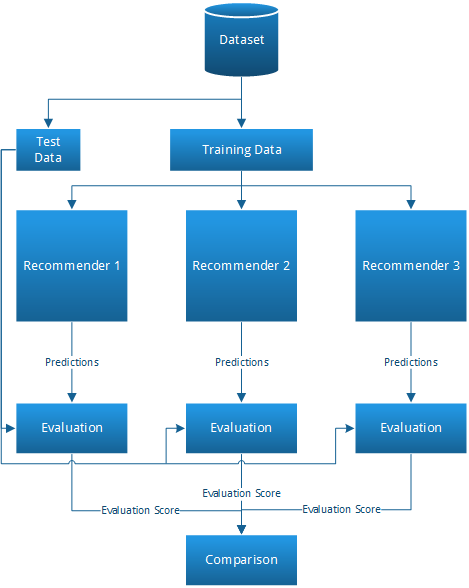
\includegraphics[scale=0.6]{image/evaluationpipeline.png}
		\caption[A Traditional Evaluation Pipeline]{A traditional evaluation pipeline for evaluating recommender systems}
		\label{figure:evaluationpipeline}
\end{figure}

Offline experiments are attractive because they require no interactions with
real users, and thus allows multiple researchers to compare a wide range of
algorithms, using the same data, at a low cost. The downside of offline
experiments is that they can answer a very narrow set of questions, typically
questions about the predictive power of the algorithm, and does not measure
other user factors.

% TODO: Already defined in preceding section. Delete?
% \paragraph{Explicit-feedback}
% The definition of explicit is defined as `stated clearly and in detail, leaving
% no room for confusion or doubt'. Explicit feedback are more precise than
% implicit feedback, but more difficult to collect since it requires active user
% involvement. One serious implication of this is that the amount of feedback
% often is scarce since many users opt not to provide any feedback. Explicit
% feedback mechanisms allow the users to unequivocally express their ratings on a
% scale (usually in the form of a Likert scale (strongly disagree --- strongly
% agree). Thus explicit feedback is able to capture both negative and positive
% feedback, while implicit feedback \emph{only} can be positive. It is worth
% noting that explicit feedback tend to concentrate on either side of the rating
% scale, as users are more likely to express their preference if they feel
% strongly for or against an item~\cite{Jawaheer2010}.
%
% \paragraph{Implicit-feedback}
% Unlike explicit feedback, we do not have any direct input from the user
% regarding their personal preferences. In particular we do not have any
% substantial evidence of which items the user dislikes, such as low ratings.
% What we do have is indications of whether a user likes an item trough clicks,
% wants and purchases. Where wants and purchases can be viewed as a form of
% explicit rating only counting positively.
% Implicit-feedback is more easily collected than explicit-feedback, and
% usually more abundant.  Types of implicit feedback include purchase history,
% browsing history, search patters, or even mouse movements. For example, a
% user who purchases many clothes from the same brand probably likes that
% brand. For a larger discussion surrounding the differences between implicit
% and explicit feedback, see Section~\ref{implicit-feedback}

\subsubsection{Validation Methods}
Validation techniques are motivated by two fundamental problems: model
selection and performance estimation. Almost all pattern recognition techniques
have one or more free parameters, and we want a way to select the
\emph{optimal} parameters or models for a given problem. Once we have chosen a
model, we wish to estimate how well it is doing.

\paragraph{The Holdout Method}
When using the holdout method you split the dataset into two groups; a training
set used to train the classifier and a test set used to estimate the error rate
of the trained classifier. The Netflix Prize Competition~\cite{Netflix}
provided a training set consisting of 100,480,507 ratings given by 480,189
users to 17,300 movies. The testset consisted of 2,817,131 items where the
ratings were unknown. The submitted predictions were scored against the true
ratings in terms of root mean squared error (RMSE), and the goal was to
minimize this error.

The holdout method has two basic drawbacks; (1) In problems with sparse
datasets we may not be able to afford the luxury of setting aside a portion of
the dataset for testing, (2) Since it is a single train-and-test experiment,
the holdout estimate can be misleading if we happen to get an `unfortunate'
split.

\paragraph{Cross-Validation}
K-fold Cross-Validation creates a K-fold partition of the dataset. For each of
the $K$ experiments, use $K-1$ folds for training and the remaining one for
testing. By setting $K=2$, this is the same as the holdout method. The estimated
error is found by taking the average error from all the experiments.

Leave-one-out is the degenerate case of K-fold Cross-Validation, where $K$ is
chosen as the total number of examples. For a dataset with $N$ examples we
perform $N$ experiments. For each experiment we use $N-1$ examples for training
and the remaining example for testing. Again, the true error is found by taking
the average error rate from the experiments.

In practice the number of folds often depends on the size of the dataset. For
large datasets, even 3-Fold Cross Validation will be quite accurate, which for
sparse datasets, one may wish to train as many examples as possible. A common
choice is $K$ value between 5 and 10.

The advantages of this methods are amongst many that the results are averaged
over the $K$ experiments. The strongest argument for using cross-validation is
the potential of using the entire training set iterativly for testing, creating
the largest possible test set for a fixed training data set.

The main disadvantage with K-fold Cross-Validation is the training algorithm
has to be run $K$ times, and thereby increasing the runtime for producing an
evaluation of the system. If the dataset is large, an increase of $K$ runs
could prove to be disadvantageous.

\paragraph{Finding optimal model-parameter settings}
Finding the optimal parameters for a model is usually a crucial task in
engineering approaches to classification and modeling tasks. An automated
approach is particularly desirable when the number of parameters is high. In
order to work well many algorithms and modeling techniques in computer science
rely on a careful choice of their parameters. The usual approach is to select
parameters based on some prior experience on the problem at hand with a limited
heuristic search of possibly optimal parameters. When such prior knowledge is
absent or cannot be directly applied to the technique being used, the optimal
parameters have to be found by \emph{blind} search, by e.g. using genetic
algorithms or some kind of exhaustive grid-search procedure.

The \emph{de facto} way of performing model selection optimization is grid
search, which is simply an exhaustive searching through a manually specified
subset of the hyperparameter space of a learning algorithm. To \emph{guide} the
grid-search one typically uses a performance metric, typically measured by
cross-validation on the training set. After evaluating the performance all the
pre-specified combinations of parameter settings, the grid search algorithm
outputs the setting that achieved the highest score in the validation
procedure.

\subsubsection{Offline Evaluation Metrics}

When evaluating a recommender system, you wish to estimate a user's
satisfaction for a given recommendation. Traditionally recommender systems have
been evaluated by means of predictive accuracy. However, there is now a widely
agreed that accurate predictions are crucial but insufficient to deploy a good
recommendation engine~\cite{Shani2011, McNee2006}. Some of the properties can
be traded-off, one such example is the trade-off between accuracy and
diversity. It is important to understand and evaluate these trade-offs and
their effect on the overall performance.
% This subsection will cover the most
% popular metrics used for offline evaluation, a discussion of evaluation
% measures for implicit feedback, and a summary of the cold-start evaluation
% methodologies found in the literature.

\paragraph{Predictive Accuracy Metrics}

Predictive accuracy metrics measure how close the predicted ratings are to the
true user ratings. More formally, the system tries to predict ratings
$\hat{r(c,i)}$ for a test set $T$ of user-item pairs $(c, i)$ for which the
true ratings are known. Traditionally, mean absolute error (MAE) has be used to
evaluate the performance of collaborative-filtering algorithms, but other
measures such as root mean squared error (RMSE) are also commonly used.

\subparagraph{Mean Absolute Error (MAE)}

MAE measures how close the predictions are to the actual outcome.

\begin{equation}
    MAE = \frac{1}{n}\sum_{i=1}^{n}{|\hat{r(c,i)}-r(c,i)|}
    \label{equation:mae}
\end{equation}

$r(c,i)$ is the actual outcome and $\hat{r}(c,i)$ is the predicted value.
As the name suggest, $MAE$ calculates the average absolute error.

\subparagraph{Root Mean Squared Error (RMSE)}

Often used to measure difference between a set of predicted values with a set of actual values.

\begin{equation}
    MSE = \frac{1}{n}\sum_{i=1}^{n}{(\hat{r(c,i)} - r(c,i))^{2}}
    \label{equation:mse}
\end{equation}

\begin{equation}
    RMSE = \sqrt{MSE}
    \label{equation:rmse}
\end{equation}

In $MSE$~\ref{equation:mse} $\hat{r(c,i)}$ is the predicted value and $r(c,i)$
is the actual value.  Both $MAE$ and $MSE$ are used to measure how correct the
predictions are compared to the actual values.  $RMSE$ is the square root of
$MSE$ and is one of the most used metrics to compare recommender algorithms in
collaborative filtering, and was the main metric used in the Netflix price
competition to evaluate the performance of the competitors recommender systems.
$RMSE$ is always bigger or equal to $MAE$, $RMSE$ penalize an error more than
$MAE$.

% \todo{maybe some sweet table of the different algorithms with their eqations and their contributions}
% \begin{table}[H]
%     \centering
%     \begin{tabular}{l|l|l}
%     	% \rowstyle{\bfseries}
%     	Metric	& Equation & About \\ \toprule
%     	MEA 			& \parbox{6cm}{\equationMEA} & safd \\	\hline
%     	RMSE 			& \parbox{6cm}{\equationRMSE} & asdf \\
%     \end{tabular}
%     \label{table:predictiveAccuracyMetrics}
%     \caption [Predictive Accuracy Metrics]{adsf}
% \end{table}

\paragraph{Measuring Usage Prediction}
\label{para:measuring_usage}
% \subsubsection{Decision Based Metrics}
In many applications the recommender system does not predict the user's
preferences of items, but tries to recommend to users items that they may use.
This is often done by giving the user a top-K set of recommendations.
In an offline evaluation of usage prediction, we typically have a dataset
consisting of items each user has used. We then select a test user, hide some
of her selections, and ask the recommender to predict a set of items the user
will use. We then have four possible outcomes for the recommend and hidden
items.

\begin{table}[H]
	\centering
	\begin{tabular}{l l l}
	\toprule
					&	Relevant			&	Not Relevant \\ \midrule
	Recommended		&	True-Positive (TP) 	&	False-Positive (FP)	\\
	Not Recommended	&	False-Negative (FN)	&	True-Negative (TN)	\\
	\bottomrule
	\end{tabular}
	\label{table:usageprediction}
	\caption[Usage prediction (Confusion Matrix)]{This table is showing the different categories recommended items can end up in.}
\end{table}

\begin{table}[H]
	\centering
	\begin{tabular}{l l}
		\toprule
		True-Positive (TP)	& The recommended item is of interest to the user \\
		False-Positive (FP)	& The recommended item is not of interest to the user \\
		False-Negative (FN)	& The item is of interest to the user, but is not recommended \\
		True-Negative (TN)	& The item is not of interest to the user, but is not recommended \\
		\bottomrule
	\end{tabular}
	\label{table:predictionCategories}
	\caption[Prediction Categories]{}
\end{table}

This model assumes that not relevant items would not have been relevant if they had been
recommended to a user. This assumption may be false, such as when the set of
not relevant items contains some interesting items that the user did not select. For
example, a user may not have relevant an items because she was unaware of its
existence, but after the recommendation exposed that item, the user can decide
to select it. We can count the number of examples that fall into each cell in
the table and compute the Precision, Recall, Fallout and $ROC$.

\subparagraph{Precision}
Precision is the fraction of retrieved items that are relevant.
\begin{equation}
    Precision = \frac{TP}{TP+FP}
    \label{equation:precision}
\end{equation}
Precision takes all recommended items into account, but it can also be evaluated at a given cut-off point, only considering the top $n$ results returned. This measure is called precision at n or P@n.

\subparagraph{Recall}
Recall is the fraction of the items that are relevant to that are successfully recommended.
\begin{equation}
    Recall = \frac{TP}{TP+FN}
    \label{equation:recall}
\end{equation}
Recall can therefore be seen as the probability that a relevant item is retrieved by the recommender.

\subparagraph{Fallout}
Fallout is the amount of retrieved items which is not relevant amongst all the non relevant items (false positive).
\begin{equation}
    Fallout = \frac{FP}{FP+TN}
    \label{equation:fallout}
\end{equation}
Fallout can therefore be looked at as the probability that a non-relevant item is recommended.

\subparagraph{F-measure}
F-measure combines the precision and the recall.
\begin{equation}
    F_\beta = \frac{(1 + \beta^2) * (Precision * Recall)}{(\beta^2 * Precision + Recall)}
    \label{equation:f-measure}
\end{equation}
Based on the value of $\beta$ F-measure will weight precision or recall more. For a $\beta$ over 1 F-measure will emphasize precision over recall, and opposite for $\beta$ between 0 and 1.

\subparagraph{Accuracy}
Accuracy is the amount of correctly recommended items over all the items.
\begin{equation}
    Accuracy = \frac{TP+TN}{TP+TN+FP+FN}
    \label{equation:accuracy}
\end{equation}

\subparagraph{Receiver Operating Characteristics (ROC)}
The $ROC$ is the recall rate ($TPR$) against the fallout rate ($FPR$).
The goal is to maximize the recall while minimizing the fallout.
\begin{equation}
    TPR(T) = \int_T^\infty P_0(T)dT
    \label{equation:tpr}
\end{equation}
\begin{equation}
    FPR(T) = \int_T^\infty P_1(T)dT
    \label{equation:fpr}
\end{equation}
$T$ is a threshold parameter.
The ROC curve is $TPR$ plotted together with $FPR$ at various $T$.

\begin{equation}
    AUROC = \int_\infty^{-\infty} TPR(T)P_0(T)dTdT
    \label{equation:auroc}
\end{equation}

Equation~\ref{equation:auroc} can be used to calculate the area under the
curve.  $AUROC$ is the probability that the recommender system will rank
positive examples higher than negative examples.  The Area Under is a commonly
used evaluation method for binary choice problems. If somebody makes random
guesses, the ROC curve should be a diagonal line stretching from (0,0) to
(1,1), as shown by the blue line in Figure \ref{fig:aucroc}, scoring an AUC of
0.5. A perfect model will score an AUC of 1.0. In practice, almost all models
will fit somewhere in between e.g. somewhat like the red or green line.

\begin{figure}[H]
\label{fig:aucroc}
  \centering
    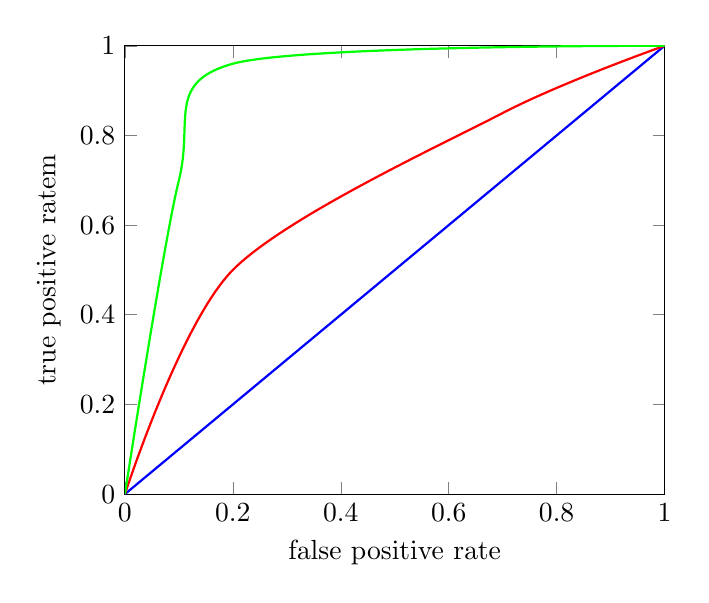
\begin{tikzpicture}
      \begin{axis}[
      	xlabel={false positive rate},
      	ylabel={true positive ratem},
      	ymin = 0, ymax=1, xmin=0, xmax=1,
      ]
      \addplot[thick,smooth,blue]{x};
      \addplot[thick,smooth,red] plot coordinates {
              (0,0)
              (0.2,0.5)
              (0.7,0.85)
              (1,1)
          };
      \addplot[thick,smooth,green] plot coordinates {
                    (0,0)
                    (0.1,0.7)
                    (0.2,0.96)
                    (1,1)
                };
      \end{axis}
    \end{tikzpicture}
    \caption{ROC curves}
\end{figure}

\subparagraph{Limitations}
\label{subp:limitations}
As mentioned by Powers et al.~\cite{powers2007}, recall, precision, F-measure have a bias.
Recall, precision and F-measure ignore performance in correctly handling negative examples, they propagate the marginal Prevalences and biases, and they fail to take account the chance level performance.
Another drawback or limitation with the measuring of user predictions is that it does not take into account the ranking of the items. To handle this, rank based metrics can be used.

\paragraph{Rank Based Metrics}
\label{para:rank_based}
Rank accuracy metrics measure the ability of a recommendation method to produce
a recommended ordering of items that matches how the user would have ordered
the same items. Shani et al.~\cite{Shani2011} lists two different approaches
for measuring the ranking accuracy: Try determining the correct order of a set
of items for each user and measure how close a system comes to this correct
order, or we can attempt to measure the utility of the system's ranking to a
user.

Herlocker et al.~\cite{Herlocker2004} argue that rank accuracy metrics may be
overly sensitive for domains where the user just wants an item that is `good
enough' (binary preferences) since the user won't be concerned about the
ordering of items beyond the binary classification. These metrics are therefore
most suitable to evaluate algorithms that are used to present ranked lists to
the user in domains where the user preferences are expressed using numerical
values.

\subparagraph{AP correlation}
\label{subp:ap_correlation}
$AP correlation$~\cite{Yilmaz:2008:NRC:1390334.1390435} measures the overall precision and is a variant of $Kendall's$ $tau$.
It counts the amount of items correctly placed in a ordered predicted rank list $list1$ and a list of the actual rank ordering of the preferences of the user $list2$.
\begin{equation}
	AP = \frac{2}{N - 1} * \sum_{i=2}^{N}{(\frac{C(i)}{i - 1})} - 1
	\label{equation:ap}
\end{equation}
How to calculate the $AP correlation$ value is shown in ~\ref{equation:ap}.
$C(i)$ is the number of items ranked correctly above rank $i$.
The value of AP is between -1 and 1, where a score of 0 means that $list1$ can be considered a randomly generated list and 1 is a perfect match with the actual list $list2$.
% \paragraph{Limitations}
% todo maybe

\label{par:accuracy_ranking}

\marginpar{if this is the setup, write a little intro}

\subparagraph{Mean Percentage Ranking (MPR)}
\label{subp:mean_percentage_ranking_}
This measure is a recall-oriented metric.
A known issue with implicit feedback is that it often lack the actual user's preference.
This approach is used to measure the user satisfaction of items in an recommended ordered list.
\begin{equation}
	MPR = \frac{\sum_{u,i}{r_{ui} * rank_{ui}}}{\sum_{u,i}{r_{ui}}}
	\label{equation:mpr}
\end{equation}
How to calculate $MPR$ is shown in~\ref{equation:mpr}.
A list of all the items for user $u$ is ordered based on the rank $rank_{ui}$ of the $u$.
Where $rank_{ui}$ is the percentile rank of item $i$ in this list for $u$.
$rank_{ui} = 0$ means that $i$ is the most preferred item for $u$.
$r_{ui}$ indicates whether $u$ has consumed $i$ or not.
This makes a $MPR$ value of 0\% to be the most preferred value, and a value of 50\% meaning a near randomly produced list.

\subparagraph{Mean Average Precision (MAP)}

\label{subp:mean_average_precision_map_}
MAP~\cite{Manning:2008:IIR:1394399} measures quality across recall levels.

\begin{equation}
	ap@n = \sum_{k=1}^{n}{\frac{P(K)}{min(m,n)}}
	\label{equation:apn}
\end{equation}
\begin{equation}
	MAP@n = \sum_{i=1}^{N}{\frac{ap@n_i}{N}}
	\label{equation:map}
\end{equation}

How to calculate the $MAP$ value is shown in~\ref{equation:map}.
\ref{equation:apn} calculates the average precision at $n$ for a user.
From \ref{equation:apn}, $P(K)$ is the precision at $k$ in the item list, $n$ is the maximum number of predicted items and $m$ is the actual length of the predicted items list.
\ref{equation:map} calculates the mean of all the values from \ref{equation:apn}.

\subparagraph{Normalized Discounted Cumulative Gain (nDCG)}
\label{subp:normalized_discounted_cumulative_gain_}

$nDCG$ measures the graded relevance of the recommended item, the ranking quality or the usefulness of the recommended item based on its rank position.
It is often used to measure the performance of web search recommendation systems.

\begin{equation}
    DCG_k = \sum_{i=1}^{k}{\frac{2^{rel_i}-1}{log_2(i+1)}}
    \label{equation:dcg}
\end{equation}

\begin{equation}
    nDCG_k = \frac{DCG_k}{IDCG_k}
    \label{equation:ndcg}
\end{equation}

How to calculate the $nDCG$ value is shown in~\ref{equation:ndcg}.
Where $k$ is the maximum amount of suggested items, and $rel_i$ is the graded relevance of the result at position $i$.
$IDCG_k$, from~\ref{equation:ndcg}, is the ideal $DCG_k$ value.
This is the result list sorted on relevance.

\subparagraph{Half-life utility~\cite{Breese:1998:EAP:2074094.2074100}}

Assume that the further down an item is in the list the less chance there is for that item to be viewed by the user.
The rate of the decaying probability is exponential.

\begin{equation}
	HL_u = \sum_{i}{\frac{\delta(i)}{2^{\frac{i-1}{\alpha-1}}}}
\end{equation}

$\delta(i)$ is 1 if the user is interested in the item at position $i$ and 0 if not.
$\alpha$ is the viewing half-life, or half-life parameter.
The half-life utility of all the users are shown in~\ref{equation:HL}

\begin{equation}
	HL = 100 * \frac{\sum_u{HL_u}}{\sum_u{HL_u^{max}}}
	\label{equation:HL}
\end{equation}

$HL_u^{max}$ is the maximum possible value of the half-life utility value.
% \paragraph{Limitations}
% todo maybe
\marginpar{some overlapping of the algorithms (not really comparing two ranked list, but still evaluating a recommender system producing ranked lists)}

\marginpar{something like this perhaps}
% paragraph accuracy_ranking (end)


\paragraph{Beyond Accuracy}
There is an emerging understanding that good recommendations accuracy alone does not give the users of the recommender system an effective and satisfying experience \cite{Herlocker2004}. The following \emph{measures} attempts to assess a recommender systems usefulness beyond being able to provide accurate recommendations to the users.

\subparagraph{Coverage}
The term coverage can refer to several distinct properties of the system. Most
commonly, the term coverage refers to the proportion of items the
recommendation system can recommend, also known as \emph{item-space coverage}.
The simplest measure of catalog coverage is the percentage of all items that
can ever be recommended. Coverage can also be the proportion of users
interactions for which the system can recommend items, known as
\emph{user-space coverage}. In many applications the recommender system may not
provide recommendations for some users due to e.g.\\ low confidence in the
accuracy of predictions for that user. In such cases one may prefer a
recommender that can provide recommendations to a wider range of users. However, an increase in coverage is only beneficial if the accuracy does not drop significantly.

\subparagraph{Perceived quality}
To gather the perceived quality the system must ask the user to examine the recommended item, and give feedback regarding the their actual interest in the recommended item.
For the feedback from the user to be as complete as possible, the system must supply the user with the reason to why the item was suggested, and the metadata of the item.
When the user has this overview of the item, the user's feedback regarding the item can produce some quality measure.
One  way of having the user to give this feedback is to re-rate the recommended item on a similar scale as the item was rated.
A rating scale from 1 to 5 is often used for both~\cite{Schafer:1999:RSE:336992.337035}.

\subparagraph{Novelty and Serendipity}
As described in Section~\ref{subsec:rec-challenges},  novelty is expected to
change over time, some times the user would like to receive recommendation on
new items, and other times recommendations closer to the user's preferences.
For the system to be able to detect these changes in preferences, and acting
accordingly would be beneficial in regards of the user's satisfaction.

\begin{equation}
    Novelty(u) = \frac{1}{N}\sum_{i=1}^{N}{1 - Knows(u,i)}
    \label{equation:novelty}
\end{equation}

In~\ref{equation:novelty} $Knows(u,i)$ represents a binary functions which
returns 1 if the user $u$ knows the item $i$, and 0 if not.  The set of items
used for the calculation is the set of recommended items for the user.

The system should be able to produce items both items known to the user, and
items unknown to the user.  For trust in the system and novelty respectively.

% TODO: How to measure serpendipity ?! (Definition happens in SotA)
% TODO: Introduce next figure.

\begin{figure}[H]
    \centering
    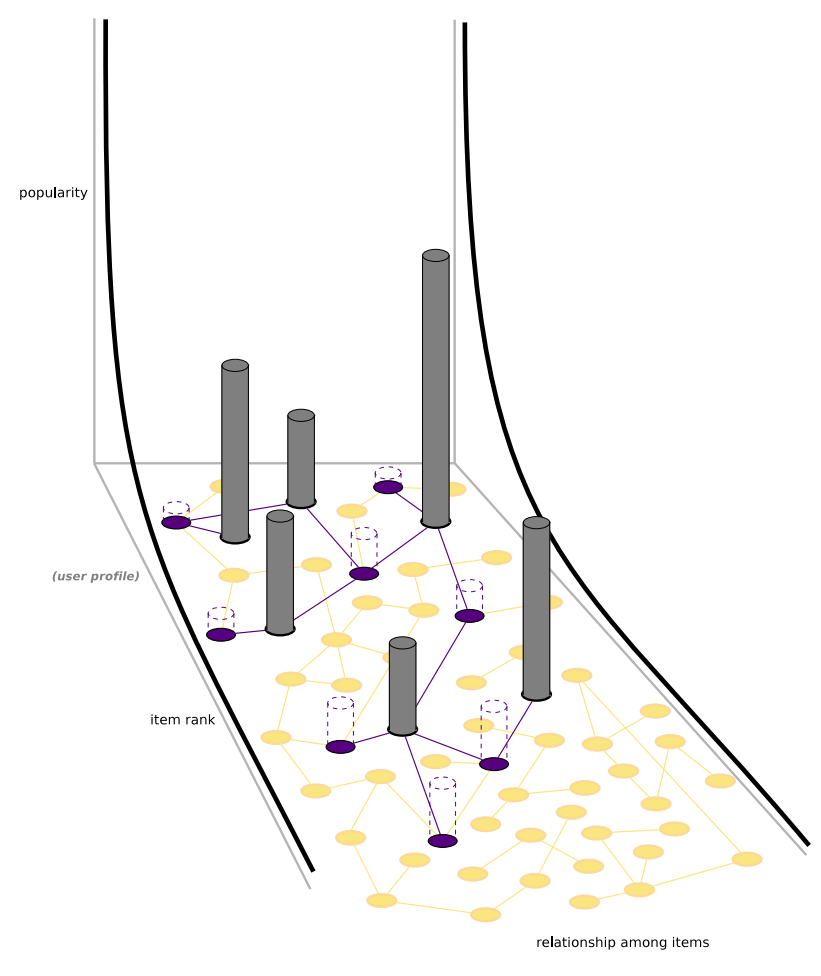
\includegraphics[scale=0.4]{image/longtailNoveltyFig.png}
    \caption{Long tail with the item similarity between items. }
    \label{figure:longtailNovelty}
\end{figure}

\marginpar{TODO: not sure if its ok to use this image (not self made) figure
from music recommendation, but long tail applies to fashion, if so extend about
longtail}

This figure show the similarity between items as a long tail graph. The gray
columns represents the user profile, the violet represents items which might be
of interest to the user, and the height is the relevance. Adapted
from~\cite{celma2008}

\subparagraph{Diversity}
Diversity is generally defined as the opposite of similarity. In some cases suggesting a set of similar items may not be as useful for the user, because it may take longer to explore the range of products. E.g. when presenting a list of 5 recommendations, the system should not recommend 5 Ralph Lauren shirts with different colors. As diversity may come at the expense of other properties such as accuracy, one should evaluate the decrease in accuracy vs. the increase in diversity.

Other evaluation methods worth knowing about includes confidence, trust, utility, robustness, adaptivity, scalability mentioned in \cite{Herlocker2004, Shani2011}.

\subparagraph{User-Centric Evaluation}
User-centric evaluation focuses on the perceived quality of the recommendation system~\cite{Pu:2011:UEF:2043932.2043962,Knijnenburg:2011:PPS:2043932.2043993}.
To gather this kind of information, user feedback is required.
User-centric evaluation is meant to handle the short comings of the offline evaluation metrics, such as predictive accuracy metrics.
User-centric evaluation can make evaluations on items which the user has not yet show interest in.
This allows user-centric evaluation to make evaluations on information about the system, such as the perceived quality and novelty of the recommendation system.
When the user feedback has been gathered the data must be analyzed.

\marginpar{move offline beyond accuracy to here maybe? }


\subsubsection{Evaluation using Implicit Feedback}
Accuracy metrics such as RMSE and MAE are not especially well suited for implicit feedback datasets, as they require knowing which items are undesired by a user~\cite{Hu2008}.
One way to handle the issue with missing negative feedback is through conversion of the implicit feedback to explicit feedback, and thereby producing a sense of negative feedback.
One issue with this is what is considered as negative feedback in the sense of implicit feedback.
The reason for a user not to access an item is not necessarily grounded in dislike, but could simply be an overlook.
On the other hand, if the user accessed the item for a short time without buying it, the user might not like it.
These questions raises the need for a different approach when wanting to measure a recommender system using implicit feedback.

Joachims et al.~\cite{Joachims07evaluatingthe} shows that clicks can be biased, and has to be interpreted relative to the order of presentation and relative to the other abstracts.

\marginpar{extend}

Two ways of measuring the system is through ranking and usage prediction described earlier.

\paragraph{Rank Based} % (fold)
	\label{par:Ranking_based}
	The ranking approach can be considered more suited to test recommendation systems using implicit feedback since a subset of the items are meant to be recommended to the user.
	This subset is usually a ranked top K list of items where the items in this list is the items the system predicts will be most liked by the user.

	One issue with this approach is that the items in the predicted top K list has to be ranked in some way, the same goes for the list this list is to be compared to.
	Thereby producing the requirement for a ranked list of preferred items from the user.
	If there is such a ranked list, ranking accuracy will help to tell how well the system is suggesting items for the user, such as~\cite{Yilmaz:2008:NRC:1390334.1390435}.
% paragraph paragraph_name (end)

\marginpar{maybe hard to differentiate between the names}

\paragraph{Accuracy Ranking} % (fold)
	\marginpar{HELGE: Språk!}
	\label{par:usage_prediction}
	When there is lack of explicit user feedback and a ranked list of the items cannot be produced, ranking the predicted list and scoring this list based on the actual user preferences can be used to evaluate the system.
	The actual user preferences are a list of binary preferences for the items.
	This list is often possible to construct from implicit feedback, but will seldom be a complete list, and most often be a list with only positives (not possible to produce not interesting).
	Some of the different approaches when dealing with implicit feedback are:
	Li et al.~\cite{deLace2010} who used $MPR$ and $MAP$ to calculate their performance.
	Pan et al.~\cite{Pan:2013:GGP:2540128.2540516} who used a set of top-k evaluation metrics: precision, recall, F1, nDCG, ROC and 1-call.
	Sindhwani et al.~\cite{Sindhwani:2010:OMC:1933307.1934641} who used roc curve and precision-recall curve to evaluate their experiments.
	Pan et al.~\cite{pan2008} who used $MAP$ and Half-life Utility.

	$nDCG$, $MAP$ and Half-life utility has a similar setup.
	They all have a decaying factor, and rewards the system in different ways for how high in the list a relevant recommended item is.

	On the other hand metrics as Precision alone has no decaying factor, and will not penalize a system with uninteresting items suggested higher in a ranked list.

	% \cite{Nati03weightedlow-rank} average squared difference
% paragraph usage_prediction (end)

	%TODO - What evaluation measures are suited for implicit feedback, and why are traditional evaluation measures such as RMSE, ... not as suitable when working with implicit feedback?

\subsubsection{Evaluation of Cold-start Recommendations}
\label{sec:cold-start-eval}
\marginpar{Helge: Pros og Cons plz}
\marginpar{Fix pros pg cons, for mye "synsing}

The cold-start problem can be considered a sub problem of coverage. The cold-start
problem occurs when the recommender system cannot draw any inferences for user or items
which it has not yet gathered sufficient information. When
evaluating the cold-start system performance one is interested in measuring the
system accuracy for these users and items.

The evaluation metric used depends on the type of feedback available.
Most experiments carried out have used \emph{traditional} explicit feedback datasets such as
MovieLens, EachMovie, Netflix etc. Accuracy metrics such as MAE~\cite{Rashid2002, Rashid2008, Massa2004,
Massa2007, Stern2009} and RMSE~\cite{Agarwal2009, Agarwal2010} are therefore
the most used ones. In the experiments where binary rating data have been used
Precision@N~\cite{Liu2011, Gantner2010}, ROC curves~\cite{Agarwal2009,
Gantner2010, Schein2002} and Area Under Curve (AUC) \cite{Liu2011, Gantner2010} seems to be the
preferred evaluation metrics.

Another way to discriminate between different recommender techniques is
coverage. The recommender system may not be able to make predictions for every
item. For this reason, it is important to measure the portion of ratings that
an RS is able to predict (ratings coverage). However, this quantity is not
always informative about the quality of a recommender system. A RS is likely to
be good at predicting nearly all the ratings for heavy users and not be able to
do the same for users who have rated few items. For this reason, one should
also compute the users coverage, defined as the portion of users which the RS
is able to predict at least one rating for. Good et al.~\cite{Good1999}
measure the item-space coverage, while Massa et al.~\cite{Massa2004,
Massa2007} measures both the item-space coverage and user-space coverage of
their methods.

Massa et.\ al~\cite{Massa2004} argue that performance measures such as Mean
Absolute User Error (MAUE) is a good measure for cold-start recommendations
since every user is taken into account once and a cold start user is as
influential as an heavy rater. Similarly, Park et al.~\cite{Park2006} measure
normalized MAE (NMAE) by macro-averaging, which first calculates the mean
average error of each users and taking the average of all users.

To simulate the cold-start scenario, different approaches have been employed:
One popular way to simulate a cold-start user scenario used by~\cite{Stern2009,
Lam2008} is to split the dataset in two disjoint sets, a training set
containing 90\% of the users and the remaining 10\% being in the test set. For
each test user one trains a model with a random subset $T\%$ of their ratings
e.g.\ $5\%$ or $75\%$, and then use the model to predict their remaining
ratings. The same methodology can also be used to simulate a cold-start item
scenario. Another highly similar way to simulate the cold-start user and
cold-start item scenario was used in~\cite{Rashid2002, Rashid2008}. For the
cold-start user scenario one selects a subset of the users with e.g.\ more than
200 ratings. One then trains the model with a subset of the ratings. In the
case of~\cite{Rashid2002} 30, 45, 60 and 90 ratings was used. After training
the model one computes the error on the hidden ratings for the same user.
Stern et. al. \cite{Stern1998} also used a similar method which they called Given $n$, in which
they trained their model using 2, 5 and 10 ratings for each test user and predict
the remaining values.

%Pros & Cons
The advantage of the latter approach is that they use a selection criteria for the test users
to avoid users with really few ratings which might be crucial on a cold-start dataset.
The obvious problem with this approach is that for cold-start datasets these users might stand for a large portion of the ratings. There are both pros and cons of using a fixed subset of ratings rather than using the percentage of ratings, the best choice will most likely depend on the dataset. Using a fixed subset of ratings would be preferable e.g. if the number number of ratings given by the users are fairly uniform.

Another \emph{simpler} approach employed by~\cite{Massa2007, Jamali2009} is to
determine a cutoff point for what is considered a cold-start user. E.g.\ that
every user with less than 5 ratings is considered a cold-start user. Then
separately measure the error on predictions made to these users.

%Pros & Cons
The problem with this approach is that it does not measure how well the recommendation quality improves as
users provide an increasing amount of ratings, giving a less detailed view of the systems performance.
The number of ratings predicted is also likely to be fairly small given a cold-start dataset.

To simulate a cold-start system scenario Agarwal et al.~\cite{Agarwal2009}
split the dataset in two using 75\% of the dataset for training and 25\% for
testing. They then train the model using 30\%, 60\% and 75\% of the data and
compare their performance on the testset.

%Pros & Cons
Good and simple model as it is likely to generate three different training sets
with different sparsity levels, which is exactly what we want to test. However,
if the training examples are drawn at random the experiment should be repeated multiple
times to avoid getting \emph{unfortunate} splits.


%Summary of articles read

%	What evaluation metrics are used?

%\cite{Rashid2008}: Accuracy metric: MAE, Expected Utility (Penalize false positives more than false negatives)
%\cite{Rashid2002}: Accuracy metric: MAE
%\cite{Massa2004}: Leave one out, MAE, MAUE, Rating Coverage, User Coverage
%\cite{Massa2007}: Leave one out, MAE, MAUE, Rating Coverage, User Coverage,
%\cite{Jamali2009}: Leave one out, Recall/Hit-ratio
%\cite{Agarwal2009}: Movie: RMSE, Yahoo: ROC curves, 5-fold cross validation
%\cite{Agarwal2010}: RMSE, True Positive Rate, True Positive Rate
%\cite{Liu2011}: Precision at N, Mean average precision, area under curve
%\cite{Park2006}: NMAE
%\cite{Good1999}: Coverage, MAE, ROC
%\cite{Stern2009}: MAE
%\cite{Ganter2010}: Precision at N (5 & 10), AUC (General ranking measure)
%\cite{Schein2002}: GROC (hit/miss rate)

%	What type of user feedback is used?

%\cite{Rashid2008}: Explicit feedback, MOVIELENS, Only users with 80 or more ratings
%\cite{Rashid2002}: Explicit feedback, MOVIELENS, Only users with 200 or more ratings
%\cite{Massa2004}: Explicit feedback, EPINIONS + Web of trust
%\cite{Massa2007}: Explicit feedback, EPINIONS + Web of trust
%\cite{Jamali2009}: Explicit feedback, EPINIONS + Web of trust
%\cite{Agarwal2009}: Explicit feedback, MovieLens + EachMovie, also incorporates user features
%\cite{Agarwal2010}: Explicit feedback + User features and bag of words rep of crawled movie data - MovieLens, Yahoo! Buzz (1 or -1), BookCrossing
%\cite{Liu2011}: Explicit feedback. Netflix...
%\cite{Park2006}: Explicit feedback, Yahoo!, MovieLens, EachMovie
%\cite{Stern2009}: MovieLens, Netflix,
%\cite{Ganter2010}: MovieLens - Binary (likes, not likes)
%\cite{Schein2002}: MovieLens, Movielens(Stripped of ratings -> implicit)

%	How do they similate the "cold-start situation"?

%\cite{Rashid2008}: Use the movies found when presenting 15, 30, 45, 60, 75 movies to provide predictions for the remaining movies in the list of each user
%\cite{Rashid2002}: Use the movies found when presenting 30, 45, 60, 90 movies to provide predictions for the remaining movies in the list of each user
%\cite{Massa2004}: Consider users who provided 2, 3 or 4 ratings, How does trust propagation of 1,2,3,4 affect rating & user coverage and predictive accurracy?
%\cite{Massa2007}: All users, cold users, heavy users, Controversial items, Black sheep, Trust propagation performance on entire dataset
%\cite{Jamali2009}: All users, cold start users (<5 ratings), recall for different neighborhood sizes
%\cite{Agarwal2009}: 25\% set aside for evaluation, train each model with 30\%, 60\%, 75\% of data, compare performance
%\cite{Agarwal2010}:
%\cite{Liu2011}: User cold start: Split users into disjoint sets (training, test). Item cold start: Split into disjoint sets
%\cite{Park2006}: Fraction of training data used [0.1 -> 1.0]. Cold-start user: Select users with more than 40 ratings in the training set and more than 1 in the test set. Split into 5, with 20\% of the users in each training set. Starting at 2 ratings, add 2 additional training set ratings per iteration until 40 ratings are added. Take the average of the 5 to compute the NMAE. Cold-start item: Items rated by more than 40 users in training data, and at least 1 user in test set. Split in 5. Starting from 2, add 2 more users per iteration. Take average NMAE from each split.
%\cite{Stern2009, Lam2008}: Divide users in two sets (90:10), train model on the 90\%. For each test user train the model on a random subset of T\% of their ratings for T = 5, T=75, then use the model to predict the remaining ratings for the user

%Clues
% http://delivery.acm.org/10.1145/570000/564421/p253-schein.pdf?ip=129.241.103.83&id=564421&acc=ACTIVE%20SERVICE&key=CDADA77FFDD8BE08%2E5386D6A7D247483C%2E4D4702B0C3E38B35%2E4D4702B0C3E38B35&CFID=419807217&CFTOKEN=62708098&__acm__=1394537427_86c608d0d7733db023faa5a09da46de7

\subsection{Online Evaluation}

Instead of doing offline evaluations on the system, one could also run large
scale experiments on a deployed system. Such experiments evaluate the
performance of recommender systems on real users which are oblivious to the
conducted experiment. The real effect of a recommender system depends on a
variety of factors such as user’s intent, the user’s context and how the
recommendations are presented to the user. All these factors are hard to
capture in an offline setting. Thus, the experiment that provides the strongest
evidence as to the true real value of the system is an online evaluation, where
the system is used by real users to perform real tasks.

\subsubsection{Online Evaluation Metrics}

Online studies in recommendations and advertisement usually measure the
click-through-rate (CTR) of the recommendations, which aligns with financial
incentives and implicitly factors in accuracy, novelty, diversity, etc.,
according to the preferences of the distribution of users.  The
click-through-rate of an algorithm is defined as the number of clicks your
recommendations get divided by the total number of recommendations that have
been made. A high CTR therefore indicates that your system is doing well.

\begin{equation}
CTR = \frac{Clicks}{Recommendations}
\end{equation}

\subsubsection{A/B Testing}
	A/B testing or bucket testing is used to test a system on live audience.
	In its' simplest form the audience is split into two groups, but it is also possible to make multiple groups of users.
	The different groups are presented with different altered versions of the system and is asked to use the system as they normally would.
	The goal is to figure out which version is producing the best results, whether it is user satisfaction or revenue.
	How the altered versions are scored is usually done trough a measure of the applications main goal, for instance with an e-commerce application where the main goal is to sell items, the score could be revenue produced by that version.

\paragraph{Example}
	In the case with the SoBazaar application, on way of doing a A/B testing on the system is as follows:
	3 groups of users are made, one with the unaltered system, one with method $A$ to produce recommendations and one with method $B$.

\subparagraph{Group Split} % (fold)
\label{par:group_split}
	The groups of users can either be selected to fit the global distribution of users, or be a set of similar minded users.
	The latter case might benefit a system where the intended goal is to specialize the system for a set of users, or actually partition the system into fitting a subsets of its' users.

\subparagraph{Group Size} % (fold)
  \label{par:group_size}
	The size of the groups depends on the amount of splits and intended stability of the system.
	The group with the original system will be the biggest group to maintain the established image of the application.
	For a system with a well established image, and a large set of faithful users, changes in the system might produce unwanted results.
	The two groups with the altered versions of the system can be of the same size to make it simpler to measure the performance of the two system against one another.

\subparagraph{System Measuring} % (fold)
\label{par:system_measuring}
	After a set period of time, the two altered versions are compared to one another and the original system.
	This is done trough measuring either the revenue produced or clicks.
	For a recommender system it is not just interesting to look at the final income number, but also if the user actually showed any interest in the products recommended for the users.
	If a larger portions of the users from version $A$ showed an increased interest in the recommended items compared to the users from version $B$, that might indicate that version $A$ is a stronger system than system $B$

\paragraph{Disadvantages}
	An issue with A/B testing is that when splitting the users into subgroups of users, these subgroups might not possess the same user properties as the complete set of groups had.
	This might lead to a biased score for the group, which might not reflect the actual score of the system when releasing it on the full set of user groups.


\subsubsection{Multi-armed bandit experiments \cite{googlebandit}}

	A multi-armed bandit is a type of experiment where:

	\begin{itemize}
	\item The goal is to find the best or most profitable action
	\item The randomization distribution can be updated as the experiment progresses
	\end{itemize}

	The "multi-armed bandit" described a hypothetical example where you face several slot machines ("one-armed bandits")
	with potentially different payouts. You wish to find the slot machine with the best payout rate, but you also want to
	maximize your winnings. The fundamental tension is between "exploiting" arms that have performed well in the past
	and "exploring" new or seemingly inferior arms in case they might perform better.

	In normal A/B testing, you will split the traffic equally between both systems, meaning that both get 50\% of the
	traffic each, all the time. When using bandits you can continuously adjust the traffic each variation receives based on its
	performance. Variations that appear to do well gets more traffic, and variations that clearly is underperforming
	gets less. The adjustments are made based on a statistical test that considers both the sample size and performance
	metrics together.

	\paragraph{Advantages}

	The main advantage of using multi-armed bandit experiments is that it usually performs better than A/B testing
	when we look at average conversion rates, which in turn will decrease the cost of the experiment.
	Saved testing time is another advantage highlighted in the Google article.

	\paragraph{Disadvantages}

	Statistical significance. Instead of sending equal traffic to each of the test pages, the page which performs
	better will start to get more traffic. If you are running tests across pages which do not get huge amounts of
	traffic, one variant can run away while the others are left in the dust without getting a fair chance. Of course,
	if your variation is performing badly you will loose some sales or conversions in the process of A/B testing,
	but that is the price one have to pay for finding out if a variation really did perform badly.

\subsection{Discussion}
The main idea behind a recommendation system is to produce a set of items which are of interest to the user.
For the system to be successful, this sets of items needs quality.
But what needs to be considered when determining the quality of the recommendations?
According to a user study~\cite{Pu:2011:UEF:2043932.2043962} the most central aspects to this quality is:

% \todo{as list or in table, or not}

\subsubsection{Perceived accuracy}
The degree of how well the user perceives the recommended items match the actual want of the user.

\subsubsection{Novelty}
The degree of new and interesting items recommended for the user.

\subsubsection{Attractiveness}
How well the recommended items are able to evoke interest or desire in the user.

\subsubsection{Diversity}
How different the recommended items are.

\subsubsection{Context compatibility}
How the system uses contextual factors to supply the recommendations with more personalized recommendations.


\subsection{The Good}
Since the data at hand is mainly implicit feedback and this data is sparse, some natural ways of approaching the evaluations task would be:

\subsubsection{MPR}
\begin{itemize}
	\item good
	\item Possible to produce a score for a recommender system which relies on implicit feedback
	\item Usable even though there are no feedback indicating undesired items
	\item Does not need a ranked list of the actual preferences of the user
	\item bad
	\item Needs distinct ranking of the different items
\end{itemize}

\subsubsection{MAP}
\begin{itemize}
	\item good
	\item Possible to produce a score for a recommender system which relies on implicit feedback
	\item Usable even though there are no feedback indicating undesired items
	\item Does not need a ranked list of the actual preferences of the user
	\item Differentiates between predicted more desired items and those that are not
	\item bad
	\item Needs distinct ranking of the different items
\end{itemize}


\subsection{The Bad}
\subsubsection{RMSE}
\begin{itemize}
	\item good
	\item Well known, so it produces a clear score of the system
	\item bad
	\item Needs the actual rating of the items
	\item Needs a predicted rating for the items
	\item Not easy to gather reliable information about undesired items trough implicit feedback
\end{itemize}


